\chapter{Error Sources Affecting Relative Quantification of CEUS} 

% \section{Abstract}
% Lorem ipsum dolor sit amet, consectetur adipiscing elit. Curabitur eget porta erat. Morbi consectetur est vel gravida pretium. Suspendisse ut dui eu ante cursus gravida non sed sem. Nullam sapien tellus, commodo id velit id, eleifend volutpat quam. Phasellus mauris velit, dapibus finibus elementum vel, pulvinar non tellus. Nunc pellentesque pretium diam, quis maximus dolor faucibus id. Nunc convallis sodales ante, ut ullamcorper est egestas vitae. Nam sit amet enim ultrices, ultrices elit pulvinar, volutpat risus.

% \section{Introduction}
% CEUS is a cheap, fast, and non-invasive imaging modality, enabling both diagnosis and monitoring of cancer, and revealing the vascular function of tissues.
% Reproducible acquisition and accurate quantification of CEUS data is of the essence to monitor cancer development, along with their vascular network.
% This is especially true when it comes to exam comparison, and in particular to compare longitudinal exams of tumors undergoing vascular-targeting therapy, i.e.~anti-angiogenic treatments. 
% Indeed, assessment of the efficiency of a therapy heavily depends on the methodology at use.
% In order to compare CEUS exams, quantification schemes should be robust to inter-exam changes, but also to acquisition context and settings.
% In a previous study, we studied the impact of inter-exam changes on perfusion parameters estimated from CEUS data, whether occurring at the experimental or physiological level.
% Additionally, a previous simulation study addressed the issue of recirculation in CEUS quantification.
% In this paper we study other sources of error, potentially affecting quantification, through a series of simulation experiment with varying factors.
% These include data intrinsic characteristics, i.e.~noise level, exam duration, sampling time; as well as quantification strategy, i.e.~analysis scale, estimation method, reference tissue selection.

\section{Introduction}
Quantification models
Simulations

\section{Theory}
\subsection{Simulation models}
In this section, the two models employed to simulate synthetic noisy CEUS data are presented.
First, the one vascular compartment model was used to generate noiseless time-intensity curves (TICs), with known physiology-related perfusion parameters.
Then, because of the multiplicative nature of the noise in ultrasound data, a parametric multiplicative noise model was used to corrupt the simulated noiseless TICs. 

\subsubsection{One vascular compartment model (OVC)}
\label{sec:OVCModel}
A vascularized tissue is considered an homogeneous compartment fed by an artery.
The vascular compartment is parameterized by tissue blood volume $V$, and tissue blood flow $F$, since the distribution of microbubbles is restricted to the vascular space~\cite{Gunn2001cx,Doury2016wn}.
An additional time-delay parameter $D$, reflecting the transit time of the contrast agent from the feeding artery to the tissue of interest, was used to fit data more accurately, thus avoiding biasing the estimation of vascular parameter. 
The mathematical expression of this model is given by equation (\ref{eq:CM}):
% \begin{equation}
% \label{eq:CM}
% C \left( t \right) = F \int_{0}^{t} C_A \left( \tau \right) \mathrm{e}^{-\frac{F}{V} \left( t - D - \tau \right)}\mathrm d \tau, \forall t \geq D, \quad 0 \textrm{ else.}
% \end{equation}
\begin{equation}
\begin{array}{rcl}
% \frac{\mathrm dC \left( t - D \right)}{\mathrm dt} &=& F \frac{\mathrm dC_A \left( t \right)}{\mathrm dt} - \frac{F}{V} C \left( t - D \right), \quad \forall t \geq D,  \\
%  &=& 0 \textrm{ otherwise.}
\dot{C} \left( t - D \right) &=& F \cdot C_A \left( t \right) - \frac{F}{V} \cdot C \left( t - D \right), \quad \forall t \geq D,  \\
 &=& 0 \textrm{ otherwise.}
\end{array}
\label{eq:CM}
\end{equation}
where $C_A$ is the AIF, $C$ is the modeled TIC, and $\dot{C}$ is the time derivative of $C$.

Given the AIF $C_A(t)$ and the TIC in a region of interest $C(t)$, three perfusion parameters can be estimated by least-squares fitting: $V$, $F$, and $D$.
Inversely, given an AIF $C_A(t)$, and the set of three perfusion parameters $V$, $F$, and $D$, the associated TIC $C(t)$ can be simulated.

\subsubsection{Multiplicative noise model}\label{sec:NoiseModel}
A multiplicative noise model following a gamma distribution enforcing unit mean was used, inspired by Barrois et al., i.e.~$\mathrm{mean}_v~p\left(v\right) = 1$, where $p\left(v\right)$ is the gamma distribution~\cite{Barrois2013}.
A unit mean distribution for a multiplicative noise ensures no bias in introduced by the noise model: it is the equivalent of a centered distribution for additive noise.

The gamma distribution is traditionally parameterized by two parameters: the shape parameter $k$, and the scale parameter $\theta$.
However, enforcing a unit mean is equivalent to set $\theta = \nicefrac{1}{k}$, the noise distribution $p\left(v\right)$ can therefore be parameterized by a single parameter, $k$, as
\begin{equation}
p\left(v\right) = \nicefrac{1}{\Gamma\left(k\right)} ~ k^k ~ v^{k-1} ~ \mathrm e^{-vk}, \forall~v \geq 0.
\end{equation}
The shape parameter $k$ controls the sharpness of the noise distribution, and is related to the standard deviation by the relation $\sigma = \nicefrac{1}{\sqrt{k}}$, allowing modulation of the noise level in simulated TICs.
Fig.~\ref{fig:recmod} shows an example of multiplicative random noise on simulated TICs for $k = 16$, corresponding to $\sigma = 0.25$.
Unless specified differently, this value of $\sigma$ was used as the default standard deviation of the noise distribution and 150 random noise sequences were generated from this distribution.

\subsection{Quantification models}
In this section we present relative quantification methods, making use of a reference tissue, derived from the previously described OVC model. 
The following methods are intended to estimate perfusion parameters from $N_T$ tissues in a single CEUS exam.
The TIC in the i$^{th}$ tissue of interest is noted $C_T^i(t)$, where $i \in \left[\![1,N_T \right]\!]$, and the TIC in the chosen reference tissue is noted $C_R(t)$. All TICs are defined for $t \in \left[ 0, L \right]$.

\subsubsection{Relative OVC model (rOVC)}
A relative OVC model can be derived from the previously presented OVC model, considering conjointly one tissue of interest with TIC $C_T^i(t)$, and one reference tissue with TIC $C_R(t)$:
\begin{equation}
\left\{
% \begin{array}{r c l}
% \frac{\mathrm dC_R \left( t - D_R \right)}{\mathrm dt} &=& F_R \frac{\mathrm dC_A \left( t \right)}{\mathrm dt} - \frac{F_R}{V_R} C_R \left( t - D_R \right), \quad \forall t \geq D_R,  \\
%  &=& 0 \textrm{ otherwise;} \\
% \frac{\mathrm dC_T \left( t - D_T \right)}{\mathrm dt} &=& F_T \frac{\mathrm dC_A \left( t \right)}{\mathrm dt} - \frac{F_T}{V_T} C_T \left( t - D_T \right), \quad \forall t \geq D_T,  \\
%  &=& 0 \textrm{ otherwise.}
% \end{array}
\begin{array}{r c l}
\dot{C_R} \left( t - D_R \right) &=& F_R \cdot C_A \left( t \right) - \frac{F_R}{V_R} \cdot C_R \left( t - D_R \right), \quad \forall t \geq D_R,  \\
 &=& 0 \textrm{ otherwise\,;} \\
\dot{C_T^i} \left( t - D_T^i \right) &=& F_T^i \cdot C_A \left( t \right) - \frac{F_T^i}{V_T^i} \cdot C_T^i \left( t - D_T^i \right), \quad \forall t \geq D_T^i,  \\
 &=& 0 \textrm{ otherwise.}
\end{array}
\right.
\label{eq:RTCM}
\end{equation}
The first equation of the system of equations (\ref{eq:RTCM}) can be rearranged as
\begin{equation}
\begin{array}{rcl}
C_A(t) &=&\frac{1}{F_{R}} \cdot \dot{C}_{R}(t - D_{R}) + \frac{1}{V_{R}} \cdot {C_{R}}(t - D_R) \quad\forall t \geq D_{R}, \\
&=& \textrm{0 otherwise.}
\end{array}
\label{eq:CACM}
\end{equation}

Replacing $C_A(t)$ in the second equation of system (\ref{eq:RTCM}) by its expression in equation (\ref{eq:CACM}), $\dot{C}_T^i(t)$ can be expressed as
\begin{equation}
\begin{array}{rcl}
\dot{C}_T^i \left(t - D_T^i\right) &= & \frac{F_T^i}{F_{R}} \cdot \dot{C}_{R}\left(t-D_R\right) + \frac{F_T^i}{V_R} \cdot C_{R} \left(t - D_{R}\right)  \\
& & \qquad - \frac{F_T^i}{V_T^i} \cdot C_{T^i} \left(t - D_{T^i}\right), \quad \forall t \geq D_T^i,\\
&=& \textrm{0 otherwise.}
\end{array}
\label{eq:RTDEF1}
\end{equation}

Defining the relative flow as $rF^i = \nicefrac{V_T^i}{V_R}$, the relative volume as $rV^i = \nicefrac{V_T^i}{V_R}$, and the rate constant in the i$^{th}$ tissue of interest as $k_T^i = \nicefrac{F_T^i}{V_T^i}$, the previous equation rewrites
\begin{equation}
\begin{array}{rcl}
\dot{C}_T^i \left(t - D_T^i\right) &= & rF^i \cdot \dot{C}_{R}\left(t-D_R\right) + rV^i \cdot k_T^i \cdot C_{R} \left(t - D_{R}\right) \\
& & \qquad - k_T^i \cdot C_{T}^i \left( t - D_{T}^i \right), \quad \forall t \geq D_T^i,\\
&=& \textrm{0 otherwise.}
\end{array}
\label{eq:RTDEF2}
\end{equation}

Assuming initial concentrations are equal to zero in both tissues, $\dot{C}_T^i$ in Eq.~\ref{eq:RTDEF2} integrates in exponential form~\cite{Yankeelov2005}, yielding
\begin{equation}
\begin{array}{rcl}
C_T^i \left( t - D_T^i \right) & = & rF^i \cdot \left( k_R - k_T^i \right) \cdot \int_{0}^{t} C_{R} \left( \tau - D_R \right) \cdot e^{- k_T^i \cdot \left( t - D_R - \tau \right)} \mathrm d \tau \\
& & \qquad + rF^i \cdot C_{R} \left( t - D_R \right) \quad \forall t \geq D_T^i, \\
&=& \textrm{0 otherwise,}
\end{array}
\label{eq:RTDEF4}
\end{equation}
where $k_R = \nicefrac{F_R}{V_R}$ is the rate constant in the reference tissue.

The latter equation, however, is not linearly solvable. 
A non-linear resolution method must therefore be used in order to estimate vascular parameters $rF^i$, $rV^i$, $k_T^i$, and $k_R$ in each of the $N_T$ tissues of interest.

\subsubsection{Linear resolution of the rOVC model (rLin)}
Alternatively, under similar assumptions, $\dot{C}_T^i$ in Eq.~\ref{eq:RTDEF2} can be integrated over time, yielding the following expression of $C_T^i$~\cite{Cardenas2013}
\begin{equation}
\begin{array}{rcl}
C_T^i \left(t - D_T^i\right) &=& rF^i \cdot C_{R}\left(t-D_R\right) + rV^i \cdot k_T^i \cdot \int_0^t C_{R} \left(\tau - D_{R}\right) \mathrm d\tau \\
& & \qquad - k_T^i \cdot \int_0^t C_{T}^i \left( \tau - D_{T}^i \right) \mathrm d\tau, \quad \forall t \geq D_T^i,\\
&=& \textrm{0 otherwise.}
\end{array}
\label{eq:RTDEF3}
\end{equation}

Assuming time delay parameters $D_T^i$ and $D_R$ are known beforehand, TICs can be time-registered, mimicking an ideal case with no delay in bolus arrival.
Variables $x^i\left(t\right)$, $y^i\left(t\right)$ are time-registered versions of the TIC in the i$^{th}$ tissue of interest and its integral.
They were defined $\forall t \in \left[ 0,\,L-D_T^i\right]$, as
\begin{equation}
\begin{array}{rcl}
x^i\left(t\right) &=& C_{T}^i\left(t\right), \\
y^i\left(t\right) &=& -\int_0^{t} C_{T}^i \left( \tau \right) \mathrm d\tau.
\end{array}
\label{eq:RTLINV1}
\end{equation}
Similarly, variables $u\left(t\right)$, $v\left(t\right)$ are time-registered versions of the reference TIC and its integral.
They were defined $\forall t \in \left[ 0,\,L-D_R\right]$, as
\begin{equation}
\begin{array}{rcl}
u\left(t\right) &=& C_{R}\left(t\right), \\
v\left(t\right) &=& \int_0^t C_{R} \left(\tau\right) \mathrm d\tau.
\end{array}
\label{eq:RTLINV2}
\end{equation}

Eq.~\ref{eq:RTDEF3} can be interpreted as an overly determined linear system of equations~\cite{Bjorck1996}, i.e.~one equation for each time sample $t$.
It therefore rewrites
\begin{equation}
x^i\left(t\right) = a^i \cdot u\left(t\right) + b^i \cdot v\left(t\right) + c^i \cdot y^i\left(t\right) \qquad \forall t \geq D_T^i,
\label{eq:RTLINF}
\end{equation}
where coefficients $a^i$, $b^i$, and $c^i$ are defined in terms of vascular parameters as
\begin{equation}
a^i = rF^i, \quad b^i = rV^i \cdot k_T^i, \quad c^i = k_T^i.
\label{eq:RTLINC}
\end{equation}

The system can be solved using a linear least-squares resolution method, yielding estimates of parameters $a^i$, $b^i$, and $c^i$ by minimization of the squared fit error $\varepsilon^i$
\begin{equation}
\argmin_{\left\lbrace a^i, b^i, c^i\right\rbrace} \varepsilon^i, \textrm{ where } \varepsilon^i = \sum_t \Big( x^i\left(t\right) - a^i\cdot u\left(t\right) + b^i\cdot v\left(t\right) + c^i\cdot y^i\left(t\right) \Big)^2.
\end{equation}
Vascular parameters of the \textbf{rLin} model can then be derived easily using
\begin{equation}
rF^i = a^i,~rV^i = \nicefrac{b^i}{c^i}, \textrm{ and } k_T^i = c^i.
\end{equation}

The linear resolution of the \textbf{rOVC} model will be referred to as \textbf{rLin} in the following.

\subsubsection{Regularized linear resolution of the rOVC model (rReg)}
Estimating $rF^i$, $rV^i$, and $k_T^i$ in $N_T$ tissues using the \textbf{rLin} model, $N_T$ values of parameter $k_R$ can be derived as a linear combination of the \textbf{rLin} model parameters:
\begin{equation}
k_R = \frac{F_R}{F_T^i}\frac{F_T^i}{V_T^i}\frac{V_T^i}{V_R} = \frac{rV^i \cdot k_T^i}{rF^i} = \frac{b^i}{a^i}
\label{eq:KR}
\end{equation}

However, there is but one reference tissue per exam, associated to a single reference TIC $C_R\left(t\right)$. 
Since parameter $k_R$ characterizes the vascular function of a single reference tissue, a unique value should be estimated per exam in order to avoid discrepancies of $k_R$ values between tissues of interest. 

The linear relation between parameters of the \textbf{rLin} model provided by Eq.~\ref{eq:KR} can be used as a constraint to ensure the $N_T$ derived values of $k_R$ are consistent across tissues.
Substituting in Eq.~\ref{eq:RTLINF} yields 
\begin{equation}
\begin{array}{rcl}
x^i\left(t\right) &=& a^i\cdot\left( u\left(t\right) + k_R\cdot v\left(t\right)\right) + c^i\cdot y^i\left(t\right),
\end{array}
\label{eq:RTREG}
\end{equation}
which rewrites 
\begin{equation}
\begin{array}{rcl}
x^i\left(t\right) &=& a^i\cdot w\left(t\right) + c^i\cdot y^i\left(t\right)
\end{array}
\label{eq:RTREG2}
\end{equation}
where $w\left(t\right)$ is a linear combination of variables $u\left(t\right)$ and $v\left(t\right)$, which were defined in Eq.~\ref{eq:RTLINV2}, 
\begin{equation}
\begin{array}{rcl}
w\left(t\right) &=& u\left(t\right) + k_R \cdot v\left(t\right),\\
&=& C_{R}\left(t-D_R\right) + k_R \cdot \int_0^t C_{R} \left(\tau - D_{R}\right) \mathrm d\tau.
\end{array}
\label{eq:RTREG3}
\end{equation}

Provided a value of parameter $k_R$, the $N_T$ linear system equations defined in Eq.~\ref{eq:RTREG} are independently solvable using a linear least-squares resolution method, minimizing the squared error, $e^i$:
\begin{equation}
\argmin_{\left\lbrace a^i, c^i \right\rbrace} e^i, \textrm{ where } e^i = \sum_{t} \Big( x^i\left(t\right) - \left[a^i\cdot w\left(t\right) + c^i\cdot y^i\left(t\right) \right] \Big)^2.
\end{equation}

Since the value of $k_R$ is unknown, and is necessary to define $w\left(t\right)$, its value must be determined.
We proposed a non-linear optimization scheme that estimates the value of $k_R$ by minimization of the normalized mean squared error, $E$:
\begin{equation}
\argmin_{k_R} E, \textrm{ where } E = \sum_i\frac{\sqrt{\nicefrac{e^i}{N^i} }}{\lvert x^i \rvert_{\infty}},
\end{equation}
$N^i$ being the number of samples in $x^i(t)$, i.e.~the number of time samples verifying $t \in \left[0,\,L-D_T^i\right]$.
Vascular parameters were then derived from the model estimates as 
\begin{equation}
rF^i = a^i,~rV^i = \frac{k_R \cdot a^i}{c^i}, \textrm{ and } k_T^i = c^i.
\end{equation}

\subsubsection{Estimation of time-delay parameters}
As stated in the presentation of the \textbf{rLin} and \textbf{rReg} models, time-delay parameters must be known beforehand, and TICs registered in time in order to solve the linear system of equations.
The determination method of the time-delay parameter, noted $D$, of a generic TIC, noted $C\left(t\right)$, used the empirical method described below.

$C\left(t\right)$ was noise-filtered twice by a moving-average filter of width 2 seconds, yielding $C_f\left(t\right)$.
The time when $C_f\left(t\right)$ reaches 20\% of its maximum value is a rough approximation that intentionally overestimates $D$, it was noted $t_{20\%}$.
$C_f\left(t\right)$ was then truncated, conserving only the part where $t \leq t_{20\%}$.
The derivative of $C_{f}\left(t\right)$, noted $\dot{C}_{f}\left(t\right)$, was approximated by convolution of the TIC with the central difference operator~\cite{Whittaker1967}. % Whittaker, E. T. and Robinson, G. "Central-Difference Formulae." Ch. 3 in The Calculus of Observations: A Treatise on Numerical Mathematics, 4th ed. New York: Dover, pp. 35-52, 1967.
Finally, assuming no oscillation occurred in the TIC prior to bolus arrival, $D$ was defined as the time at which the derivative $\dot{C}_{f}\left(t\right)$ reaches 20\% of its value at $t = t_{20\%}$:
\begin{equation}
\exists D\in\Re^+,~D \leq t_{20\%}\,\wedge\,\dot{C}_{f}\left(D\right) = 20\% \times \dot{C}_{f}\left(t_{20\%}\right).
\end{equation}

\section{Materials and Methods}
\subsection{Simulations of CEUS data}
\subsubsection{Simulation process}
Regional perfusion parameters were derived from experimental data fitted with the OVC model presented in Section~\ref{sec:OVCModel}.
The arterial input function was estimated in the image using the segmentation method presented in Chapter~\ref{chapter:PMB}.
A log-normal model was fitted to the resulting arterial curve for noise-filtering purposes. 
Regional enhancement curves were simulated using the same model, along with the estimated model parameters and arterial input function.

\subsubsection{Varying factors}
\paragraph{Noise level}
The influence of noise was investigated by varying parameter $\sigma$, i.e.~the standard deviation of the multiplicative noise level presented in Section~\ref{sec:NoiseModel}.
$\sigma$ was varied linearly with increments of 0.05 from 0, corresponding to a noiseless conditions, to 0.5, corresponding to high noise conditions.
For each noise level, 150 random noise sets following the multiplicative gamma noise model were generated.
Example time-intensity curves with varying noise levels are displayed in Figure~\ref{fig:simNoise}.

\paragraph{Exam duration}
Various exam durations were investigateds by varying the number of samples in the simulated data.
More precisely, the exam duration was varied from 50 seconds to 165 seconds with 5 seconds increments.

\paragraph{Sampling period}
Simulated noiseless enhancement curves were resampled using varying sampling periods to study the impact of this parameter on the accuracy and precision of the estimation.
The sampling period was varied from 0.1 to 1.0 second with 0.1 increments, this range is representative of the acquisition settings that can be found in contrast-enhanced ultrasound studies.

\paragraph{Reference tissue}
The reference tissue can be represented functionally by the parameters of the OVC model, i.e.~$V_R$, $F_R$, and $k_R = \dfrac{F_R}{V_R}$.
The impact of these parameters on the accuracy and the precision of the quantification process using the \textbf{rLin} and the \textbf{rReg} models was investigated.
In particular, the tissue blood volume, the tissue blood flow of the reference tissue were varied by scaling either or both of them by $\dfrac{1}{2}$, $\dfrac{2}{3}$, $1$, $\dfrac{3}{2}$, and $2$.
Because of the relation between the three parameters, they cannot be varied individually.
It is however possible to fix either of the parameters while varying the two others.
The disks at the bottom Figure~\ref{fig:simRef} shows the various values of the perfusion parameters used to simulate the reference tissue enhancement curve, the center disk being the original value obtained from experimental data.

\begin{figure}
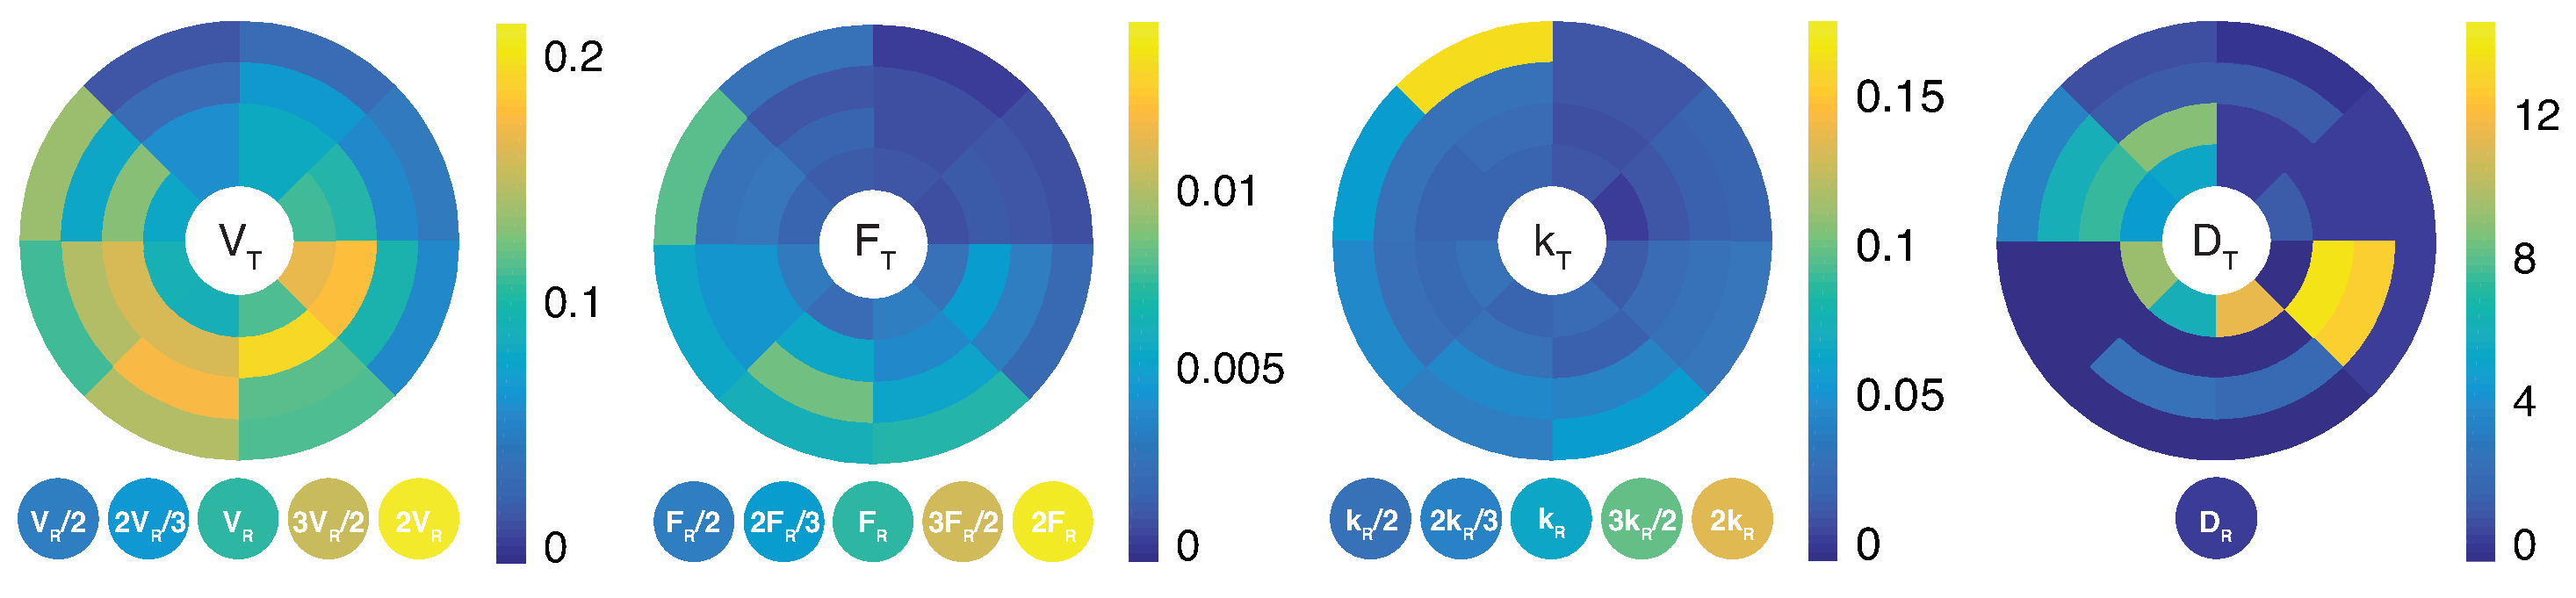
\includegraphics[width=\linewidth]{simRef.eps}
\caption{Absolute perfusion parameters used for simulation with the OVC model, i.e.~tissue blood volume, $V_T$ and $V_R$, tissue blood flow, $F_T$ and $F_R$, tissue rate constant, $k_T$ and $k_R$, and time delay, $D_T$ and $D_R$. Bullseye view of the parameters in the 32 tumor regions. The bottom disks represent the parameters used to simulated the reference tissue region, the center disk being the original value used for all experiments. The other disks are, from left to right, the half, two third, three half, and double of the original value, used to study the influence of the reference tissue.}
\label{fig:simRef}
\end{figure}

\paragraph{Number of regions}
Various regional segmentation were performed varying the number of tumor regions as powers of two, ranging from 1 to 32.
For each segmentation, the parameters of the OVC model were estimated using the mean enhancement curve in each tumor and reference region, as well as an estimate of the arterial input function derived from the image. 
Figure~\ref{fig:simReg} shows the simulated values of the perfusion parameters for the various segmentations with a varying number of regions. 
The absolute perfusion parameters of the OVC model were used to derive the parameters of the rOVC model using the definitions of Eq.~\ref{eq:RTDEF2}.
The derived parameters were then used as ground truth to evaluate the accuracy of the perfusion parameters estimated using the \textbf{rLin} and the \textbf{rReg} models.

\begin{figure}
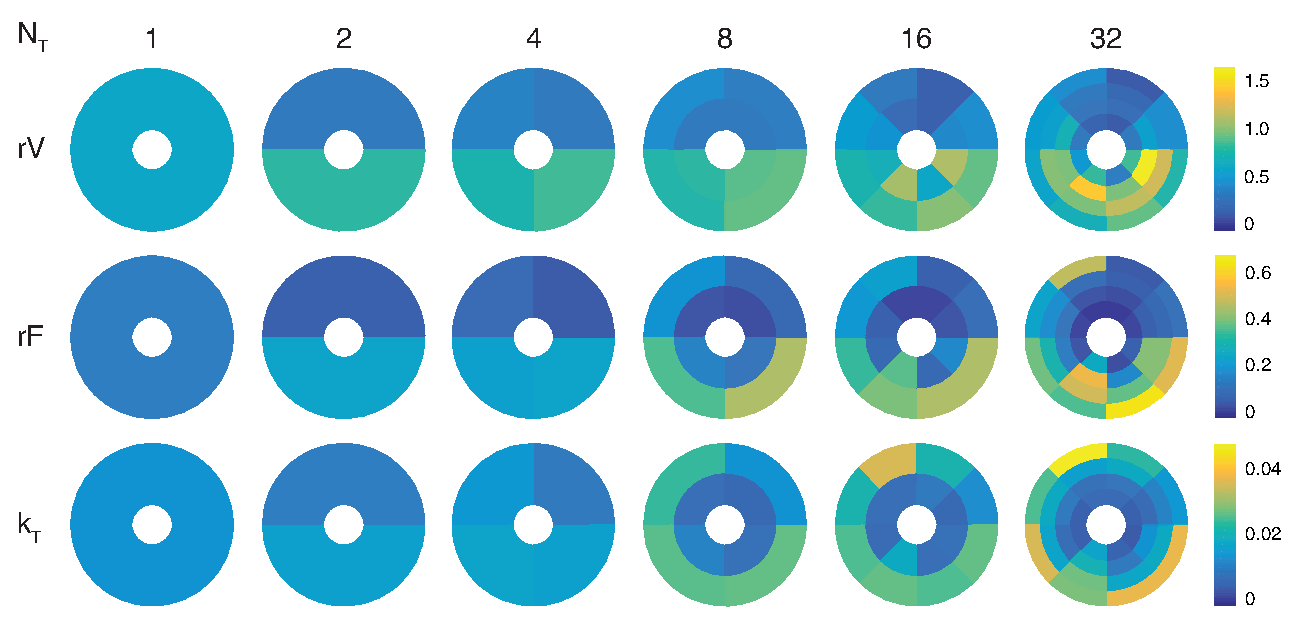
\includegraphics[width=\linewidth]{simReg_sim.eps}
\caption{Relative perfusion parameters used for simulation varying the number of tumor regions $N_T$ from 1 (left) to 32 (right), i.e.~relative tissue blood volume, $rV$, relative tissue blood flow, $rF$, tissue rate constant, $k_T$.}
\label{fig:simReg}
\end{figure}

\subsection{Data analysis}\label{sec:dataAnalysis}
The accuracy and the precision of the parameters estimated using the \textbf{rLin} and the \textbf{rReg} models were respectively investigated through the median value and either the standard deviation or the interquartile range of the relative estimation error over 150 random noise samples.
The relative estimation error of parameter $\theta$, noted $rE_{\theta}$, is expressed in percent and defined as
\begin{equation}
rE_{\theta} = 100 \times \frac{\theta_{est}-\theta_{sim}}{\theta_{sim}}
\end{equation}
i.e.~the difference between the estimated parameter $\theta_{est}$ and the simulated parameter $\theta_{sim}$, normalized by the simulated value.

\section{Results}
\paragraph{Noise level}
Figures~\ref{fig:noise_rV} to \ref{fig:noise_kR} show the relative estimation error of the relative tissue blood volume ($rV$, Figure~\ref{fig:noise_rV}), relative tissue blood flow (Figure~\ref{fig:noise_rF}), and rate constants in the tumor (Figure~\ref{fig:noise_kT}) and reference  (Figure~\ref{fig:noise_kR}) tissues obtained using the \textbf{rLin} and \textbf{rReg} models, as a function of the noise level simulated in the data, i.e.~the standard deviation of the multiplicative noise model.

Expectedly, for the four parameters of both models, the interquartile range of the relative estimation bias increased with the noise level, and no relation was found between the noise level and the median value of the relative estimation error.
In terms of relative tissue blood volume (see Figure~\ref{fig:noise_rV}), the two models were hardly differenciable.
Inside a given region, the median relative estimation error value can be different with a slight advantage for the \textbf{rLin} model, but the precision of the estimation is however generally comparable.
Additionally, the \textbf{rReg} model makes the estimation bias of $rV$ more consistent across regions.
Regarding relative blood flow (see Figure~\ref{fig:noise_rF}), the \textbf{rLin} model was generally more accurate than the \textbf{rReg} model. 
However the estimation of $rF$ was less precise and more sensitive to noise using the \textbf{rLin} model.
In terms of the rate constant in tumor tissues (see Figure~\ref{fig:noise_kT}), the \textbf{rReg} model proved both more accurate and more precise than the \textbf{rLin} model.
Indeed, the \textbf{rReg} model exhibited an extremely consistent estimation bias across regions, with an average of -3\%, and a lower sensitivity to noise.
The \textbf{rLin} model on the other hand, yielded estimates of $k_T$ with highly variable biases, with median biases reaching 40\% in one of the regions, and overestimating the parameter in some regions while underestimating it in others.
A common value of the rate constant in the reference tissue (see Figure~\ref{fig:noise_kR}), $k_R$, was estimated for all tumor regions using the \textbf{rReg} model.
The regularized model underestimated $k_R$ by 5\% in average in our experiments and exhibited a rather low sensitivity to noise. 
Oppositely, the estimates of the \textbf{rLin} model were extremely inconsistent across regions, and were more sensitive to noise in most regions.

\begin{figure}
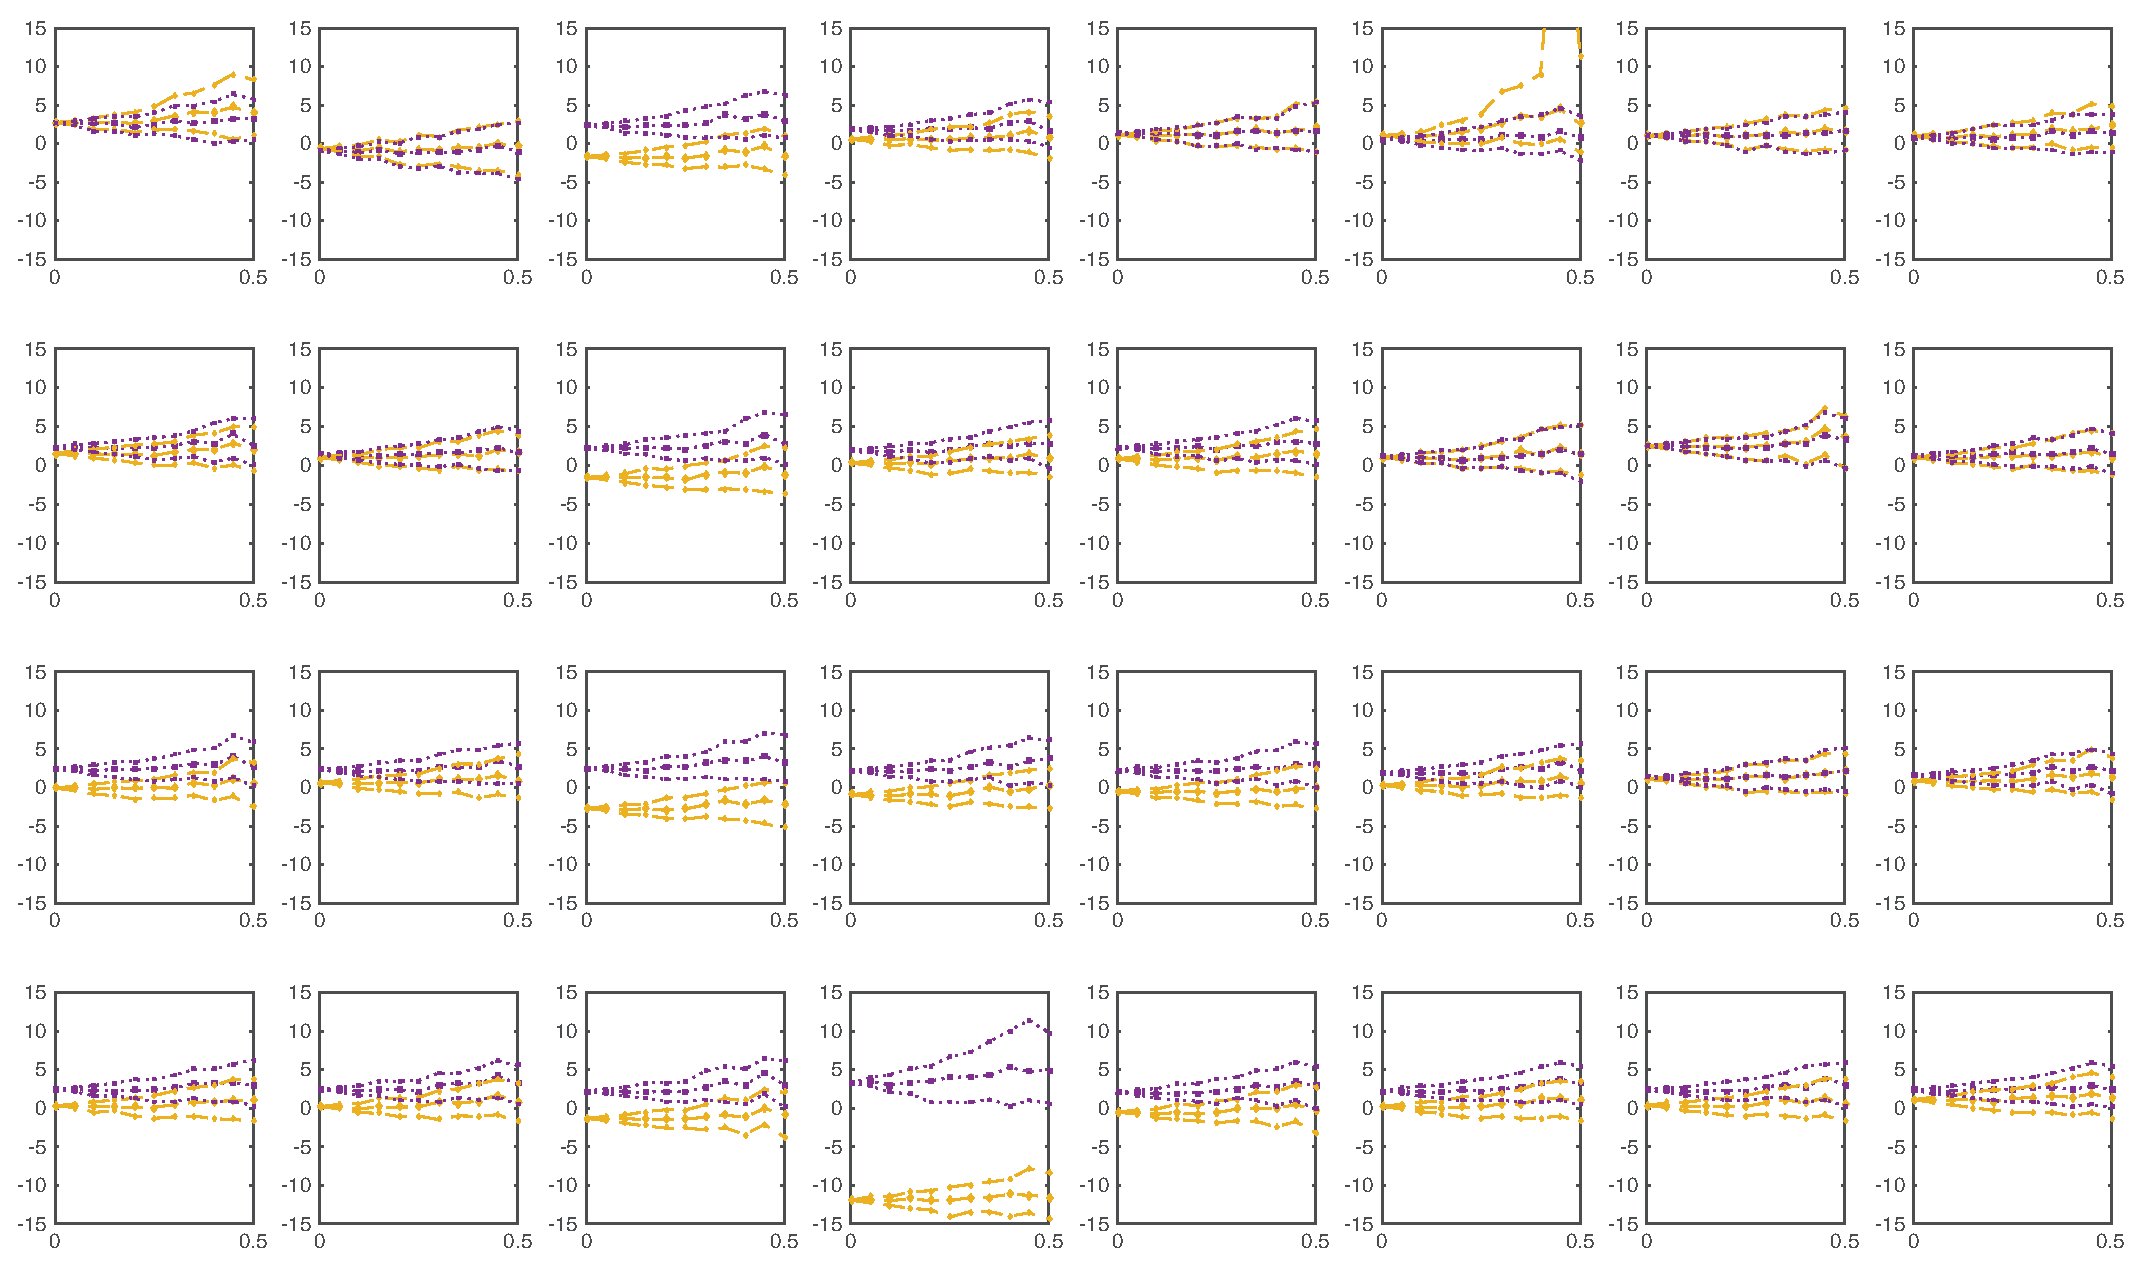
\includegraphics[width=\linewidth]{simNoise_rV.eps}
\caption{Median (large symbols) and first and third quartiles (small symbols) of the relative estimation error for the relative blood volume ($rV$) estimated using the \textbf{rLin} (yellow diamonds) and \textbf{rReg} (purple squares) models, as a function of the noise level.}
\label{fig:noise_rV}
\end{figure}

\begin{figure}
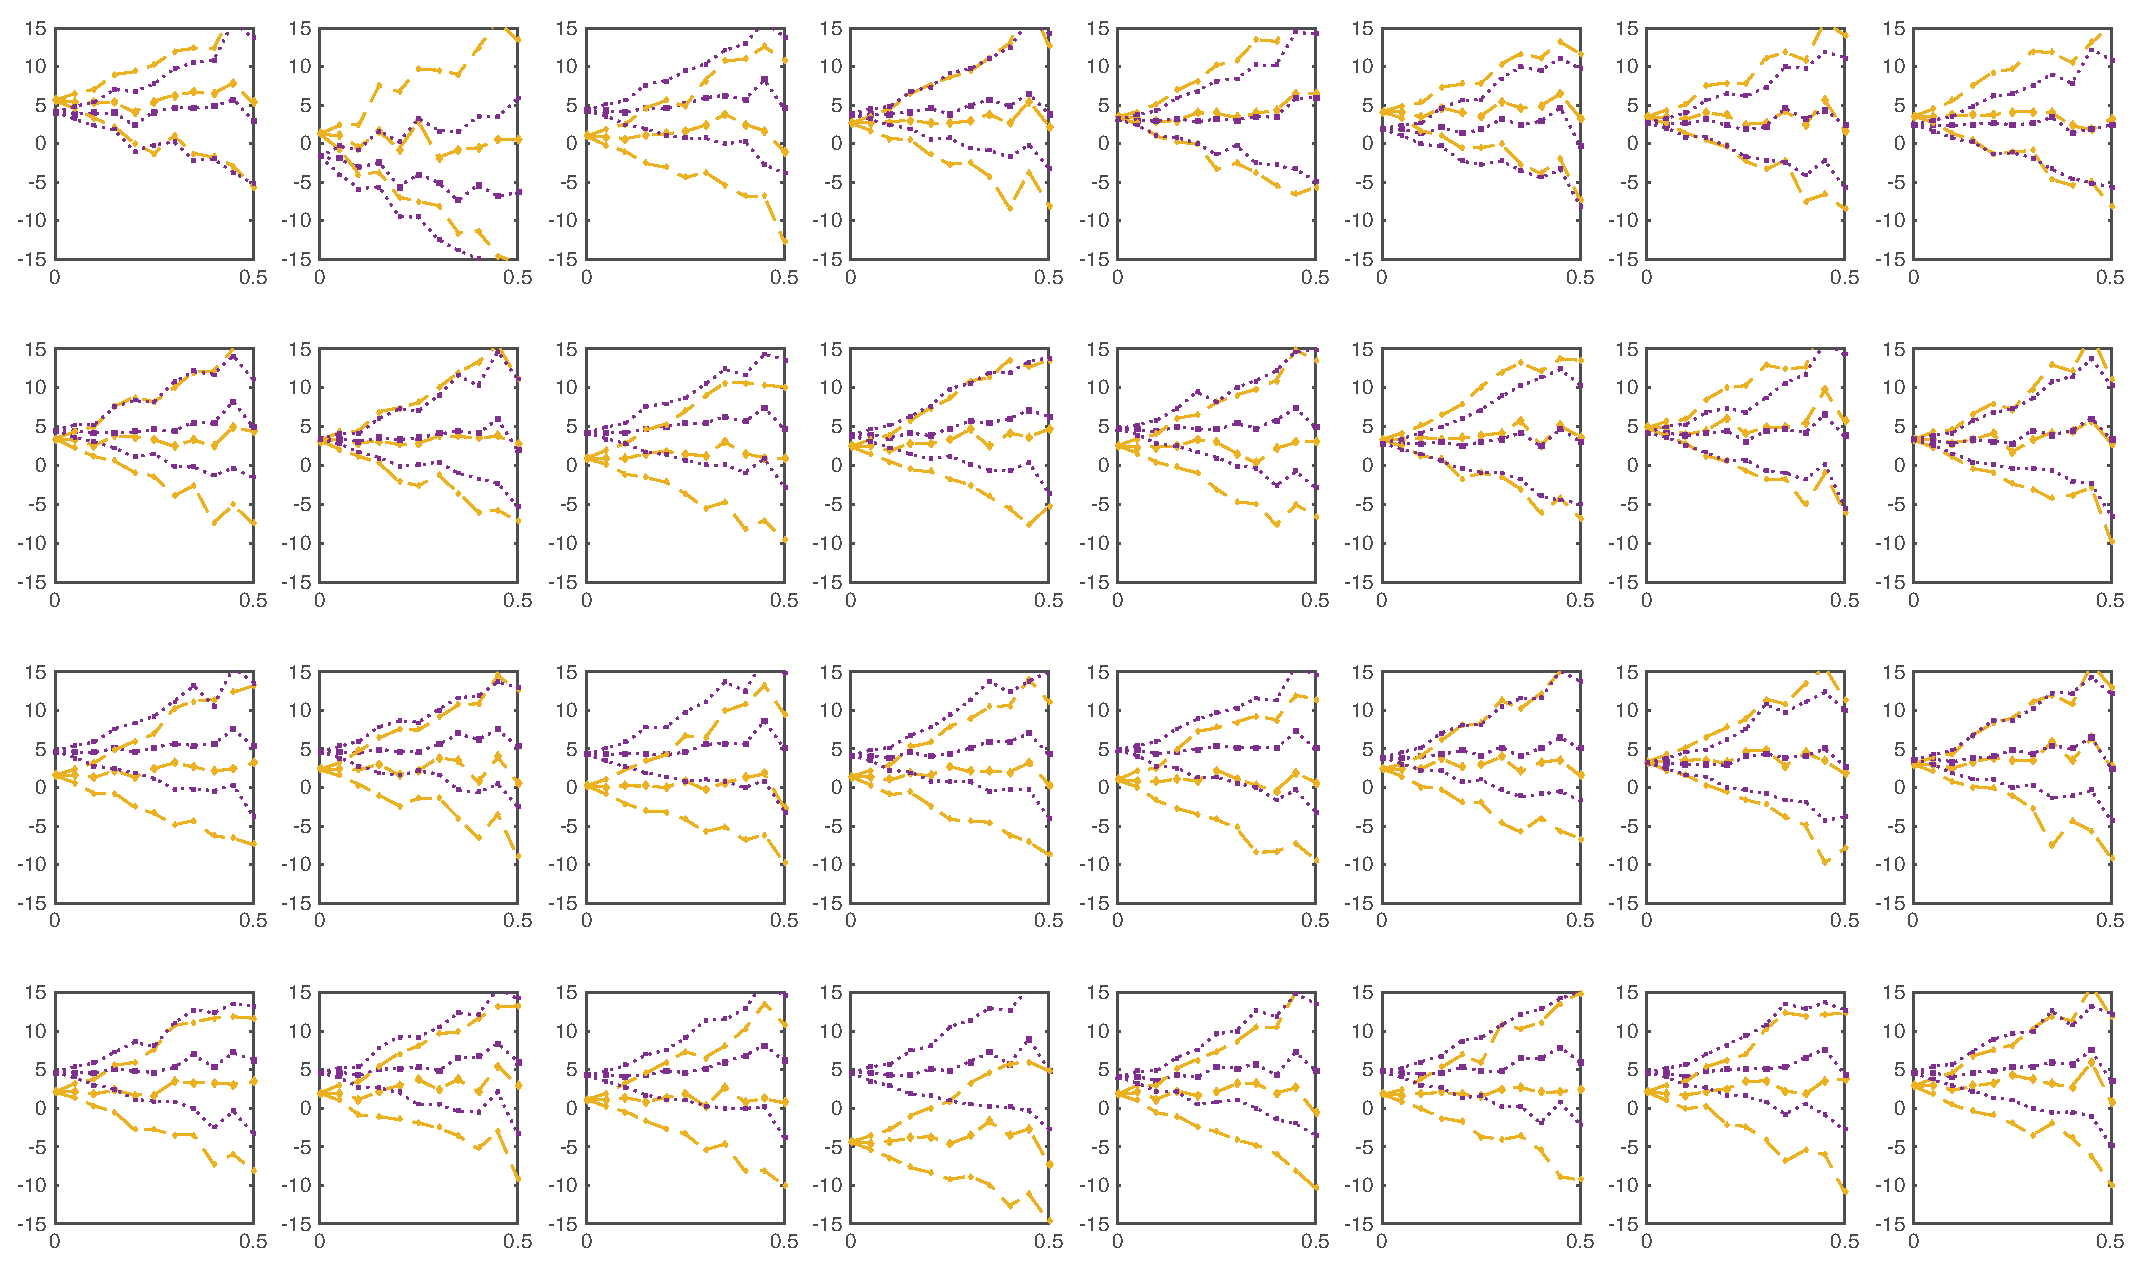
\includegraphics[width=\linewidth]{simNoise_rF.eps}
\caption{Median (large symbols) and first and third quartiles (small symbols) of the relative estimation error for the relative blood flow ($rF$) estimated using the \textbf{rLin} (yellow diamonds) and \textbf{rReg} (purple squares) models, as a function of the noise level.}
\label{fig:noise_rF}
\end{figure}

\begin{figure}
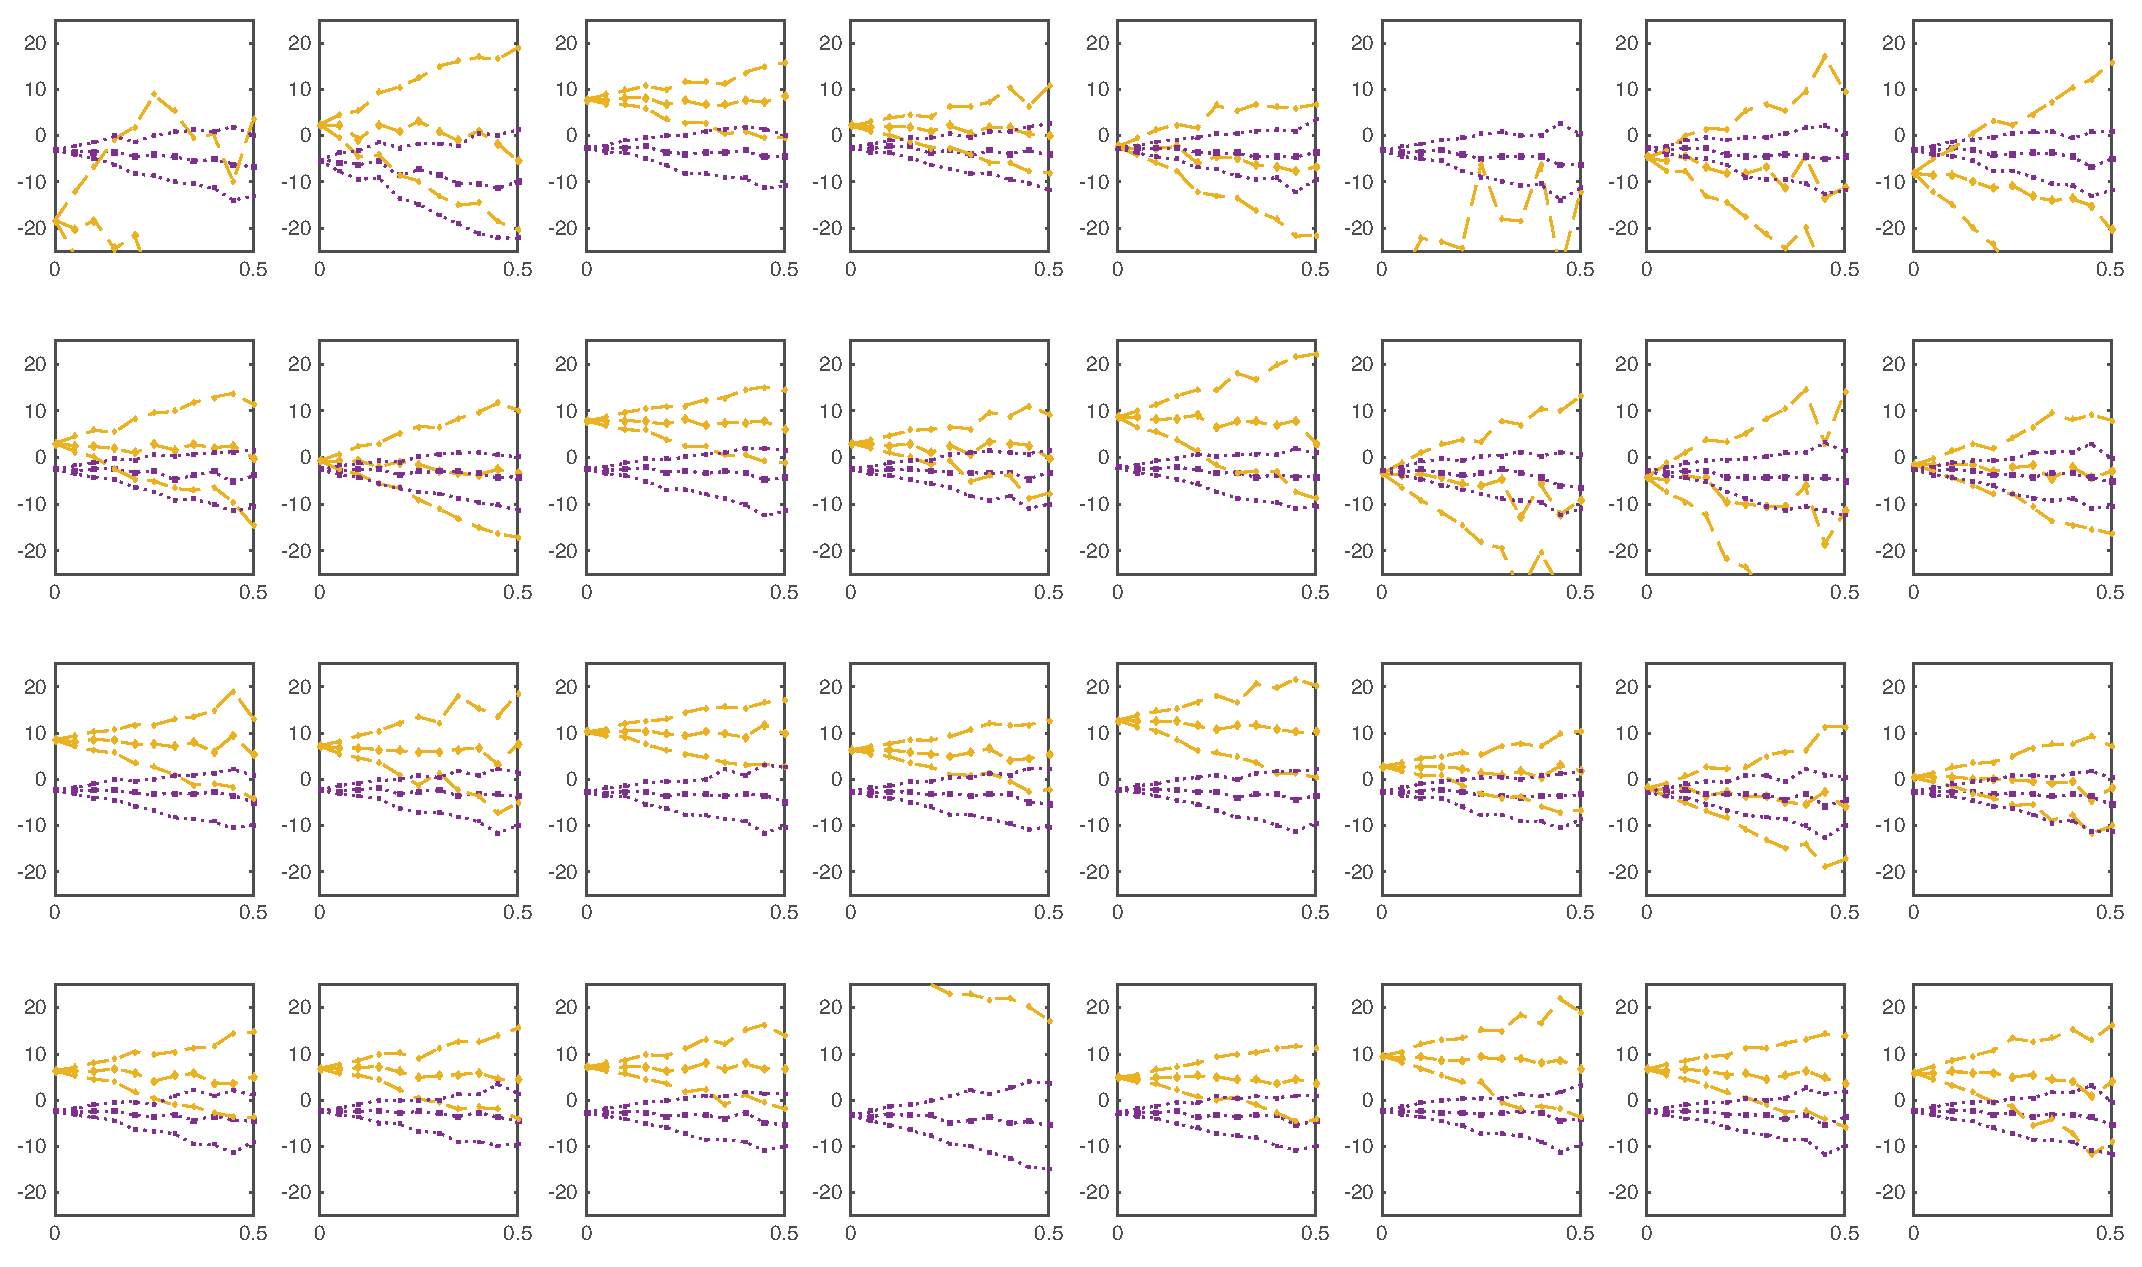
\includegraphics[width=\linewidth]{simNoise_kT.eps}
\caption{Median (large symbols) and first and third quartiles (small symbols) of the relative estimation error for the rate constant in the tumor ($k_T$) estimated using the \textbf{rLin} (yellow diamonds) and \textbf{rReg} (purple squares) models, as a function of the noise level.}
\label{fig:noise_kT}
\end{figure}

\begin{figure}
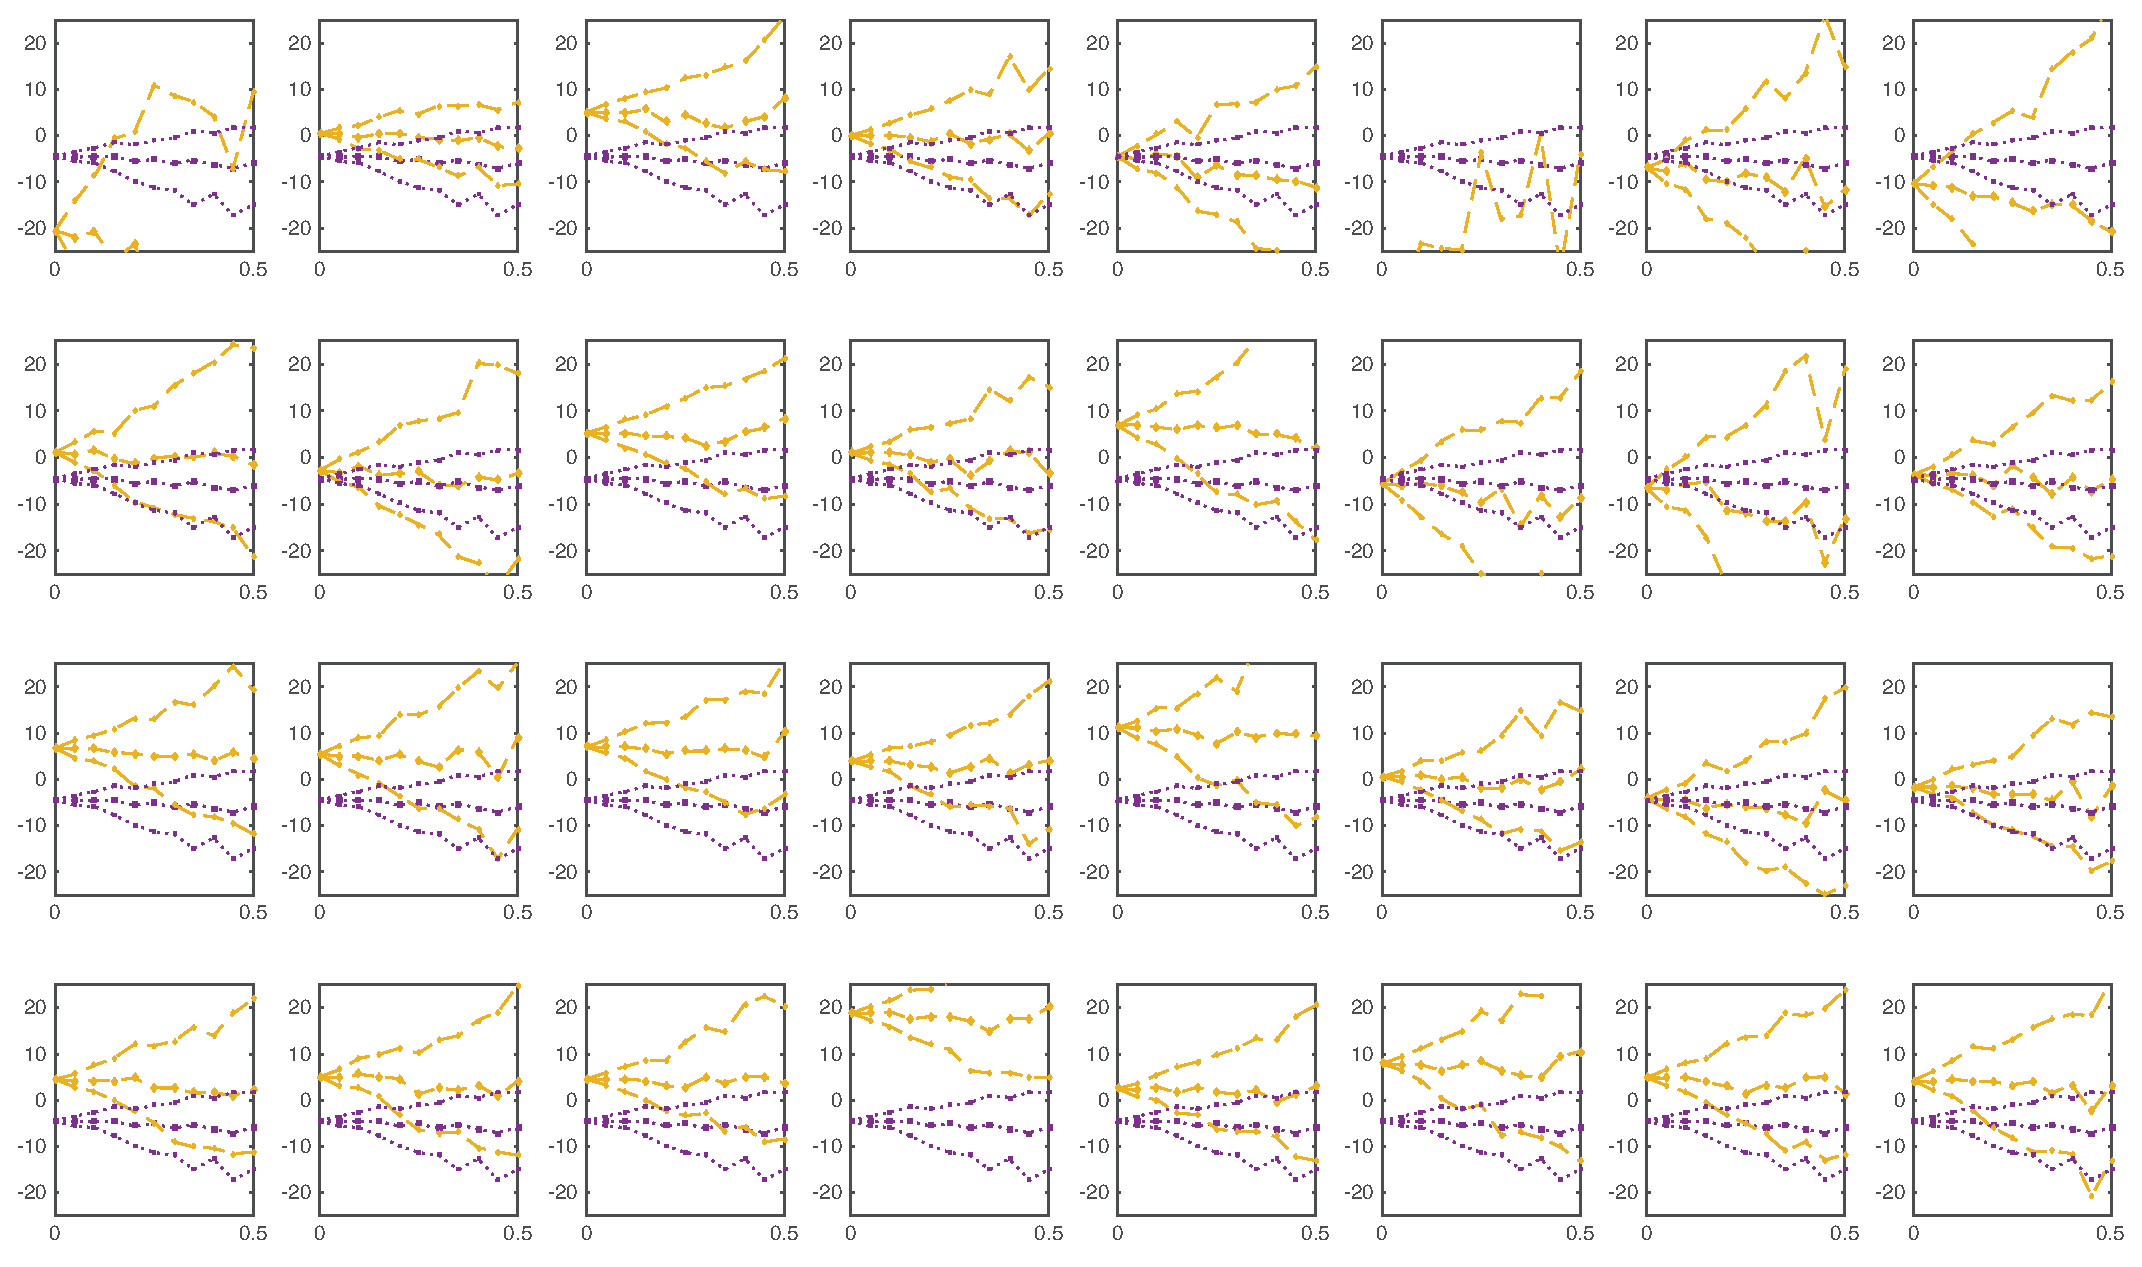
\includegraphics[width=\linewidth]{simNoise_kR.eps}
\caption{Median (large symbols) and first and third quartiles (small symbols) of the relative estimation error for the rate constant in the reference tissue ($k_R$) estimated using the \textbf{rLin} (yellow diamonds) and \textbf{rReg} (purple squares) models, as a function of the noise level.}
\label{fig:noise_kR}
\end{figure}

\paragraph{Exam duration}
Figures~\ref{fig:examDuration_rV} to \ref{fig:examDuration_kR} show the impact of the exam duration on the relative estimation error of the perfusion parameters of the \textbf{rLin} and \textbf{rReg} models, i.e.~relative tissue blood volume (Figure~\ref{fig:examDuration_rV}), relative tissue blood flow (Figure~\ref{fig:examDuration_rF}), and rate constants in the tumor (Figure~\ref{fig:examDuration_kT}) and in the reference tissue (Figure~\ref{fig:examDuration_kR}).
In Figures~\ref{fig:examDuration_rV} to \ref{fig:examDuration_kR}, each plot represents a tumor region, i.e.~the top row corresponds to the outer rim and the bottom row to the inner rim, the columns correspond to the clockwise ordering of the regions on a rim starting with the left region above the horizontal line.

Regarding relative blood volume (see Figure~\ref{fig:examDuration_rV}), the \textbf{rReg} model was able to estimate the parameter accurately, and to reach a steady state with exams as short as 80 seconds.
Oppositely, the \textbf{rLin} model only yielded accurate estimates using the whole exam duration, i.e.~165 seconds, and at the exception of one region it overall underestimated $rV$.
Comparably, the relative blood flow (see Figure~\ref{fig:examDuration_rF}) was steadily estimated using the \textbf{rReg} model with exams as short as 50 seconds, despite an average overestimation of less than 4\%.
The estimates of $rF$ given by the \textbf{rLin} were found more sensitive to the duration of the exam, and generally overestimated $rF$ for very short exams, the bias decreasing with exam duration.
And then, past some duration threshold, which variable from one region to another, the bias increased linearly with the exam duration.
Regarding the rate constant in the tumor (see Figure~\ref{fig:examDuration_kT}), the \textbf{rLin} model was unable to accurately estimate the parameter for incomplete exams, and exhibited strong biases in short exams, again varying from one exam to another. 
The \textbf{rReg} model was able to steadily and uniformely estimate parameter $k_T$, despite a tendency of the median relative estimation error to slightly decrease with the exam duration for exams lasting more than 100 seconds.
Moreover, the estimation of $k_T$ was more precise using the \textbf{rReg} model.
For both models, the bias in the estimation of $k_R$, the rate constant in the reference tissue (see Figure~\ref{fig:examDuration_kR}), was strongly correlated to the bias in the estimation of $k_T$.


\begin{figure}
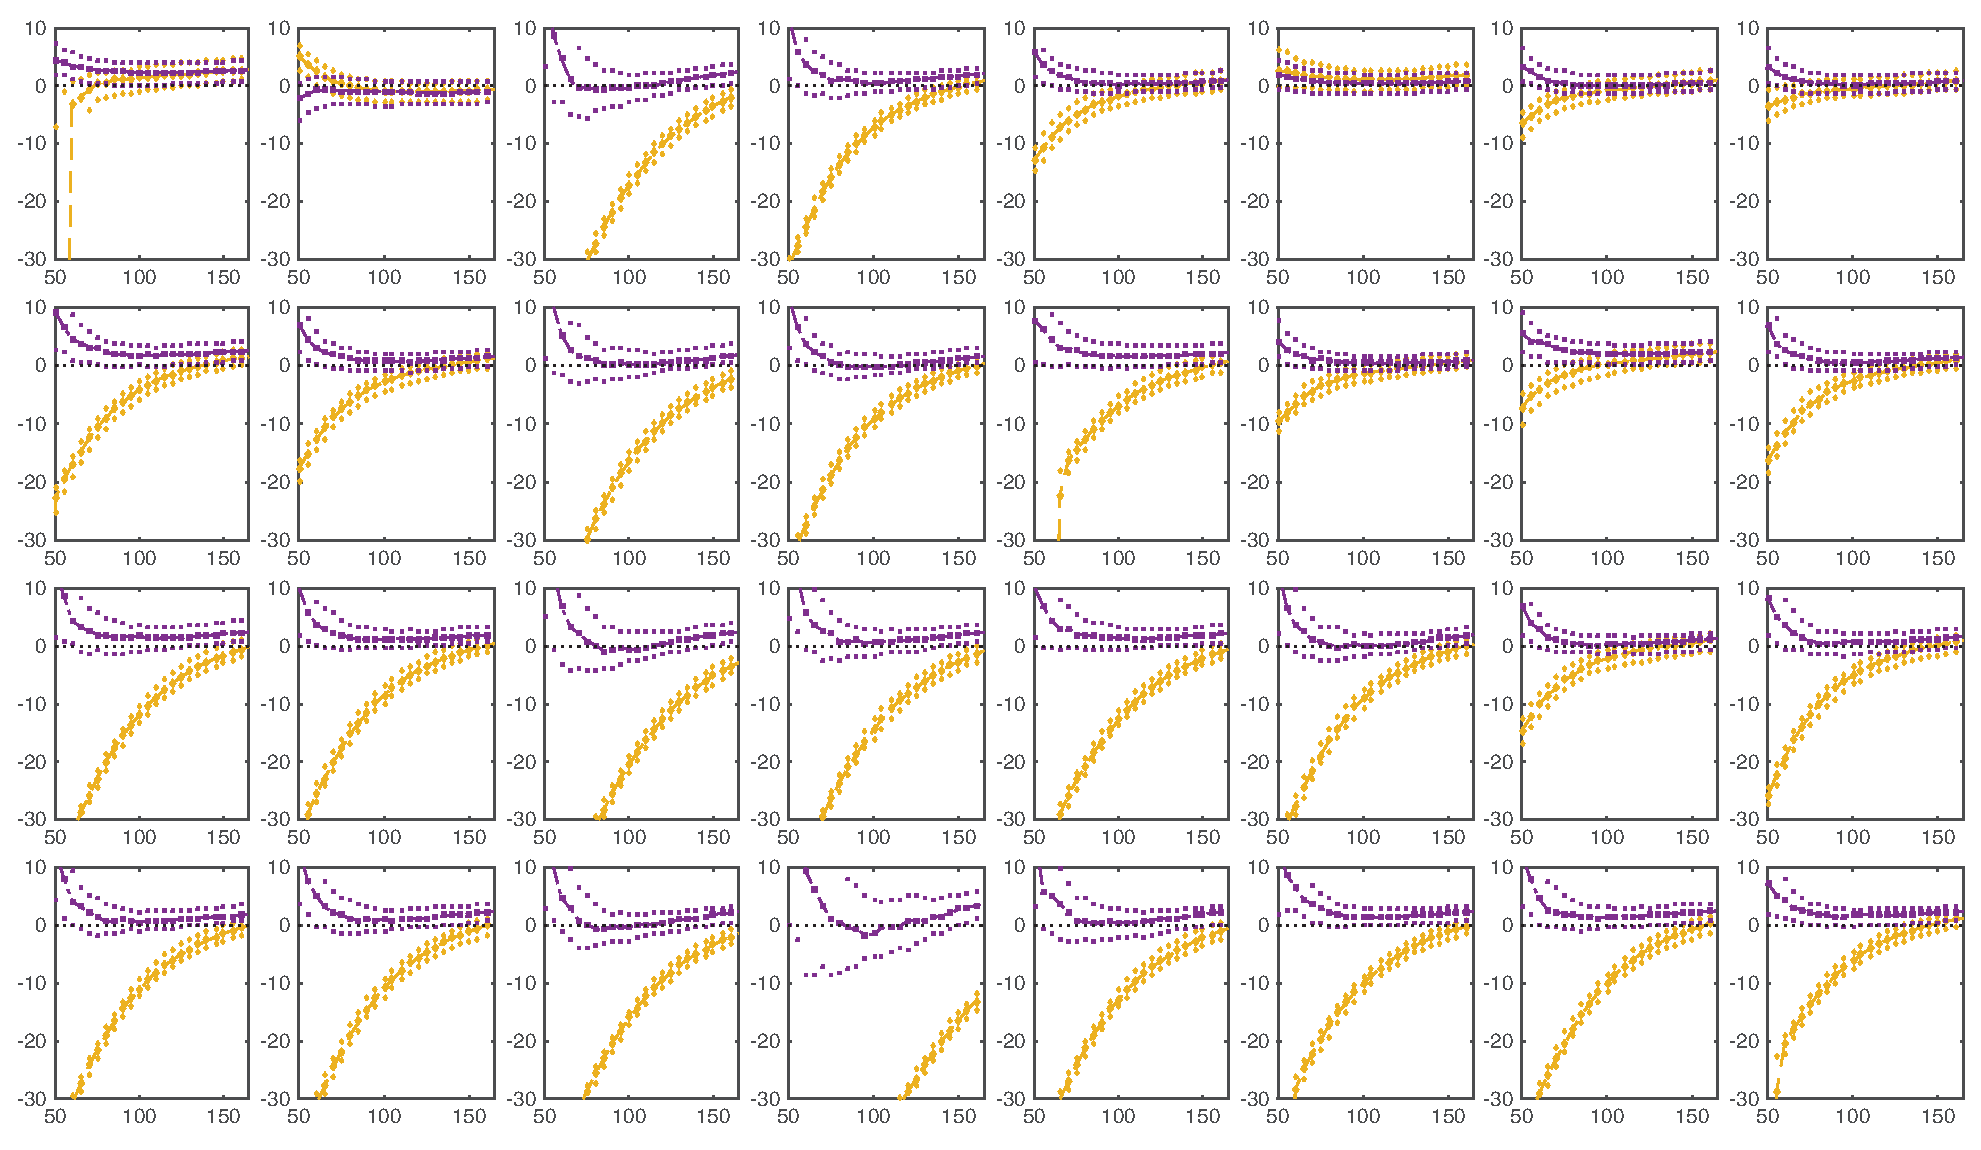
\includegraphics[width=\linewidth]{simSamples_rV.eps}
\caption{Median (large symbols) and first and third quartiles (small symbols) of the relative estimation error for the relative blood volume ($rV$) estimated using the \textbf{rLin} (yellow diamonds) and \textbf{rReg} (purple squares) models, as a function of the exam duration.}
\label{fig:examDuration_rV}
\end{figure}

\begin{figure}
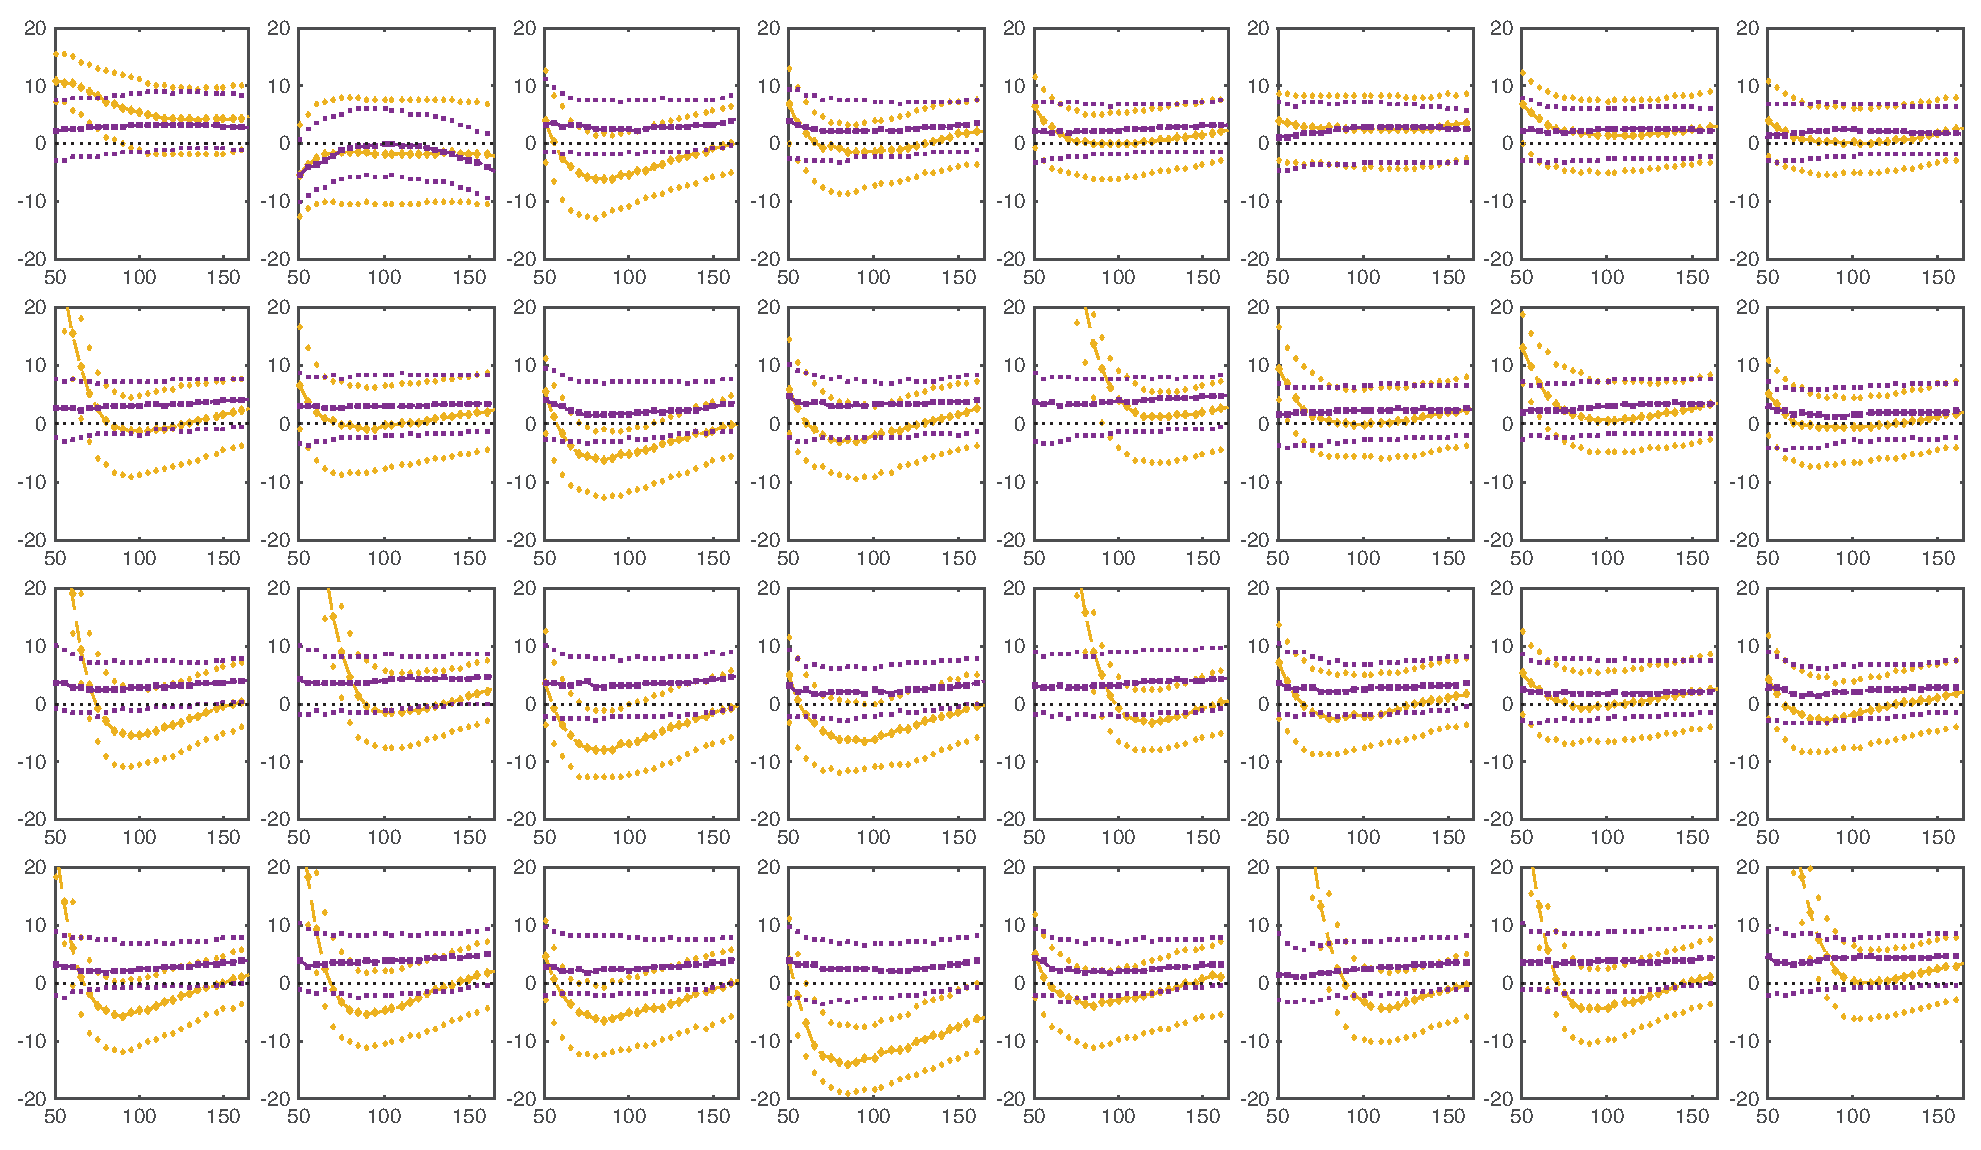
\includegraphics[width=\linewidth]{simSamples_rF.eps}
\caption{Median (large symbols) and first and third quartiles (small symbols) of the relative estimation error for the relative blood flow ($rF$) estimated using the \textbf{rLin} (yellow diamonds) and \textbf{rReg} (purple squares) models, as a function of the exam duration.}
\label{fig:examDuration_rF}
\end{figure}

\begin{figure}
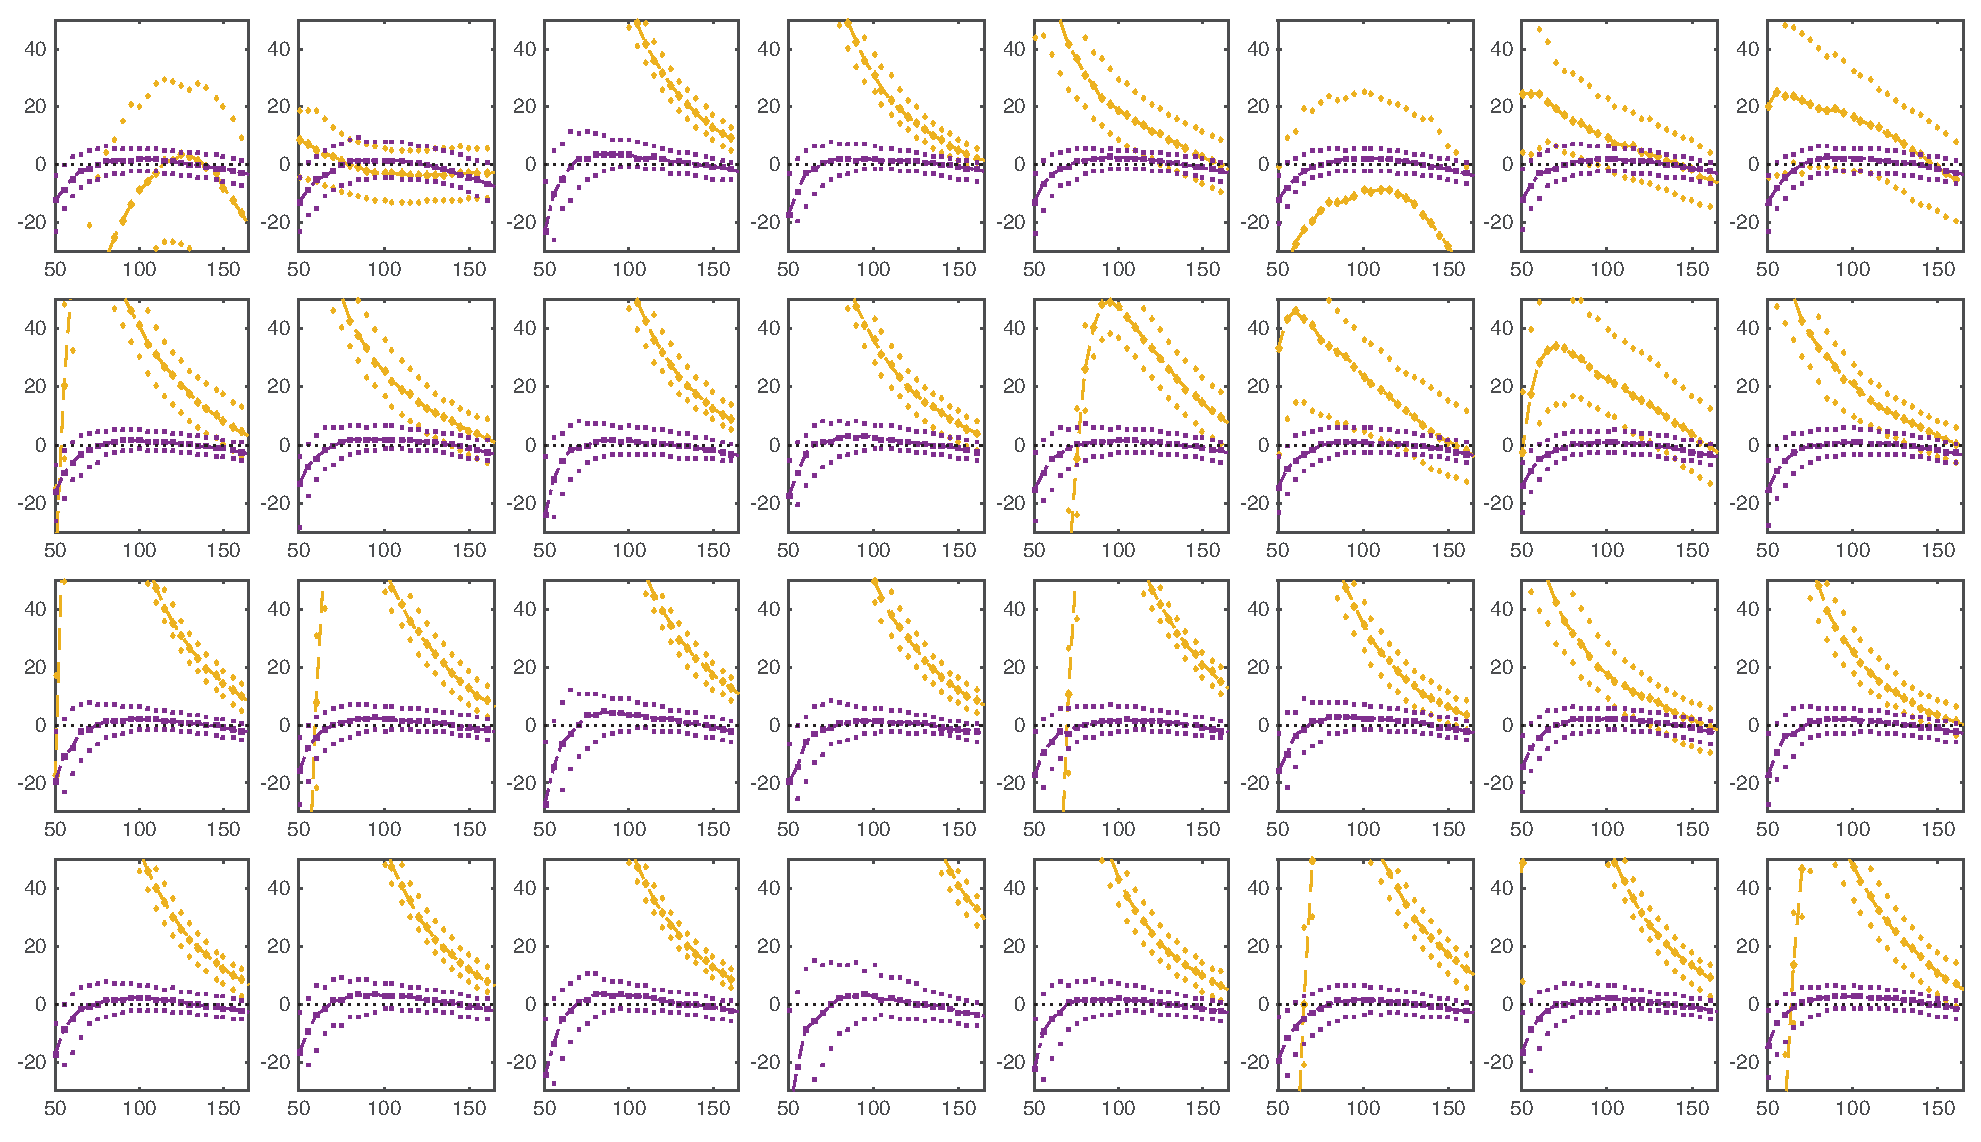
\includegraphics[width=\linewidth]{simSamples_kT.eps}
\caption{Median (large symbols) and first and third quartiles (small symbols) of the relative estimation error for the rate constant in the tumor ($k_T$) estimated using the \textbf{rLin} (yellow diamonds) and \textbf{rReg} (purple squares) models, as a function of the exam duration.}
\label{fig:examDuration_kT}
\end{figure}

\begin{figure}
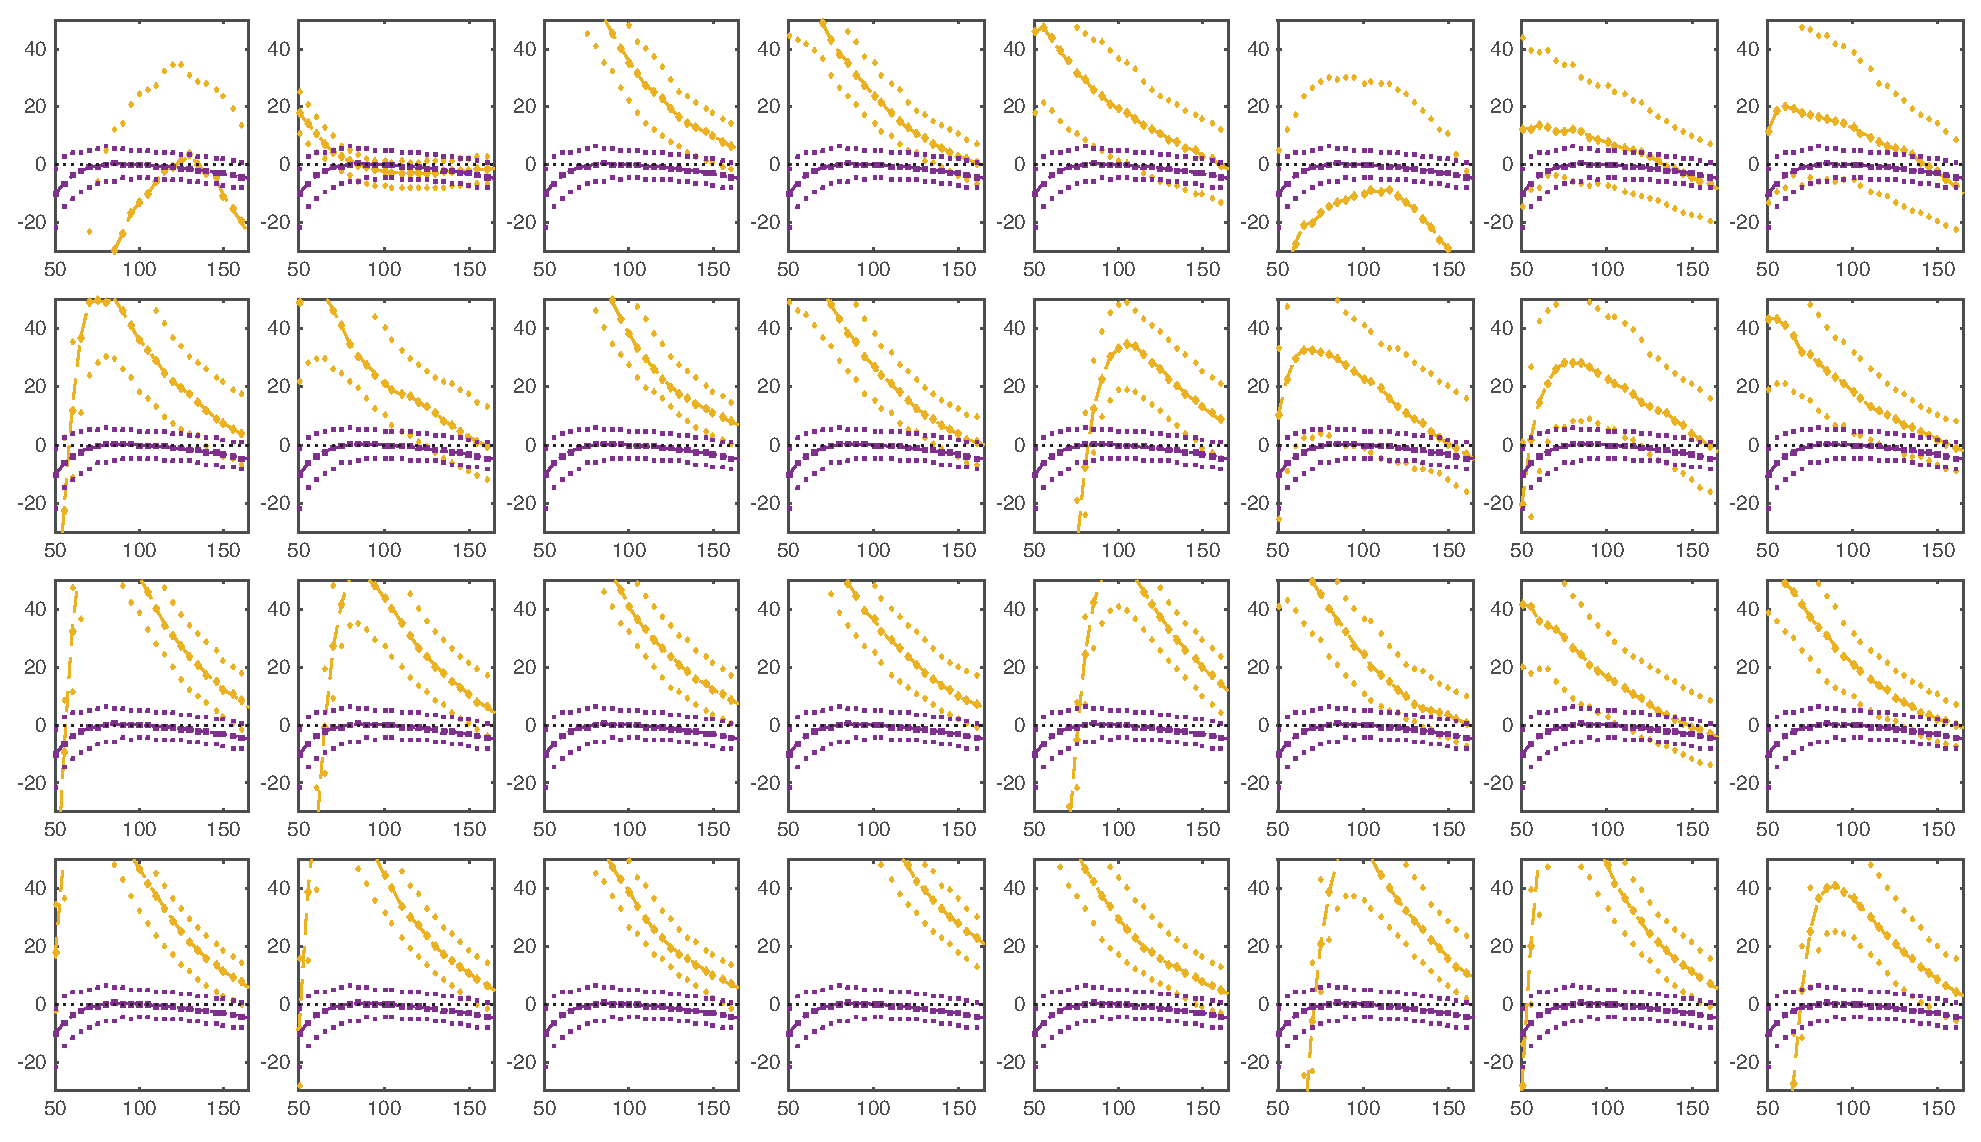
\includegraphics[width=\linewidth]{simSamples_kR.eps}
\caption{Median (large symbols) and first and third quartiles (small symbols) of the relative estimation error for the rate constant in the reference tissue ($k_R$) estimated using the \textbf{rLin} (yellow diamonds) and \textbf{rReg} (purple squares) models, as a function of the exam duration.}
\label{fig:examDuration_kR}
\end{figure}


\paragraph{Sampling period}
Figures~\ref{fig:sampling_rV} to \ref{fig:sampling_kR} show the impact of the sampling period on the relative estimation error of the perfusion parameters of the \textbf{rLin} and \textbf{rReg} models, i.e.~relative tissue blood volume (Figure~\ref{fig:sampling_rV}), relative tissue blood flow (Figure~\ref{fig:sampling_rF}), and rate constants in the tumor (Figure~\ref{fig:sampling_kT}) and in the reference tissue (Figure~\ref{fig:sampling_kR}).
In Figures~\ref{fig:sampling_rV} to \ref{fig:sampling_kR}, each plot represents a tumor region, i.e.~the top row corresponds to the outer rim and the bottom row to the inner rim, the columns correspond to the clockwise ordering of the regions on a rim starting with the left region above the horizontal line.

Varying the sampling period over the investigated range, i.e.~from 0.1 to 1 second, did not have a significant impact on the accuracy of the estimation of the relative tissue blood volume parameter using both the \textbf{rLin} and \textbf{rReg} models (see Figure~\ref{fig:sampling_rV}), and only a slight decrease in precision was observed for larger sampling period.
Similarly to the varying noise level experiments, the bias in the estimation bias of $rV$ was more consistent across regions using the \textbf{rReg} model, with the median relative estimation errors generally inferior to 4\%.
The estimates of $rF$, the relative tissue blood flow, exhibited a tendency to decrease with increasing sampling period, especially in regions with large simulated $k_T$ values. 
While in most regions the estimates of $rF$ from the \textbf{rReg} model get closer to zero for large sampling periods, one region underestimated the parameter by more than 20\%.
The estimates of $rF$ from the \textbf{rLin} model exhibited a similar trend, but in addition they were overall more sensitive to the sampling period in terms of precision, and less consistent across regions.
In terms of rate constant in the tumor (see Figure~\ref{fig:sampling_kT}), the \textbf{rReg} model yielded consistent negative biases across regions, and generally yielded more precise estimates than the \textbf{rLin} model.
For both models, a slight decrease of the estimates of $k_T$ with the sampling period was observed for both models in most regions, but stronger negative slopes were observed in regions with larger simulated $k_T$.
The rate constant in the reference tissue was estimated consistently across tumor regions using the \textbf{rReg} model (see Figure~\ref{fig:sampling_kR}), and despite a slight underestimation, the estimation was overall more accurate and precise with this model.
Indeed, the estimation of $k_R$ using the \textbf{rLin} model was extremely imprecise in some regions.

\begin{figure}
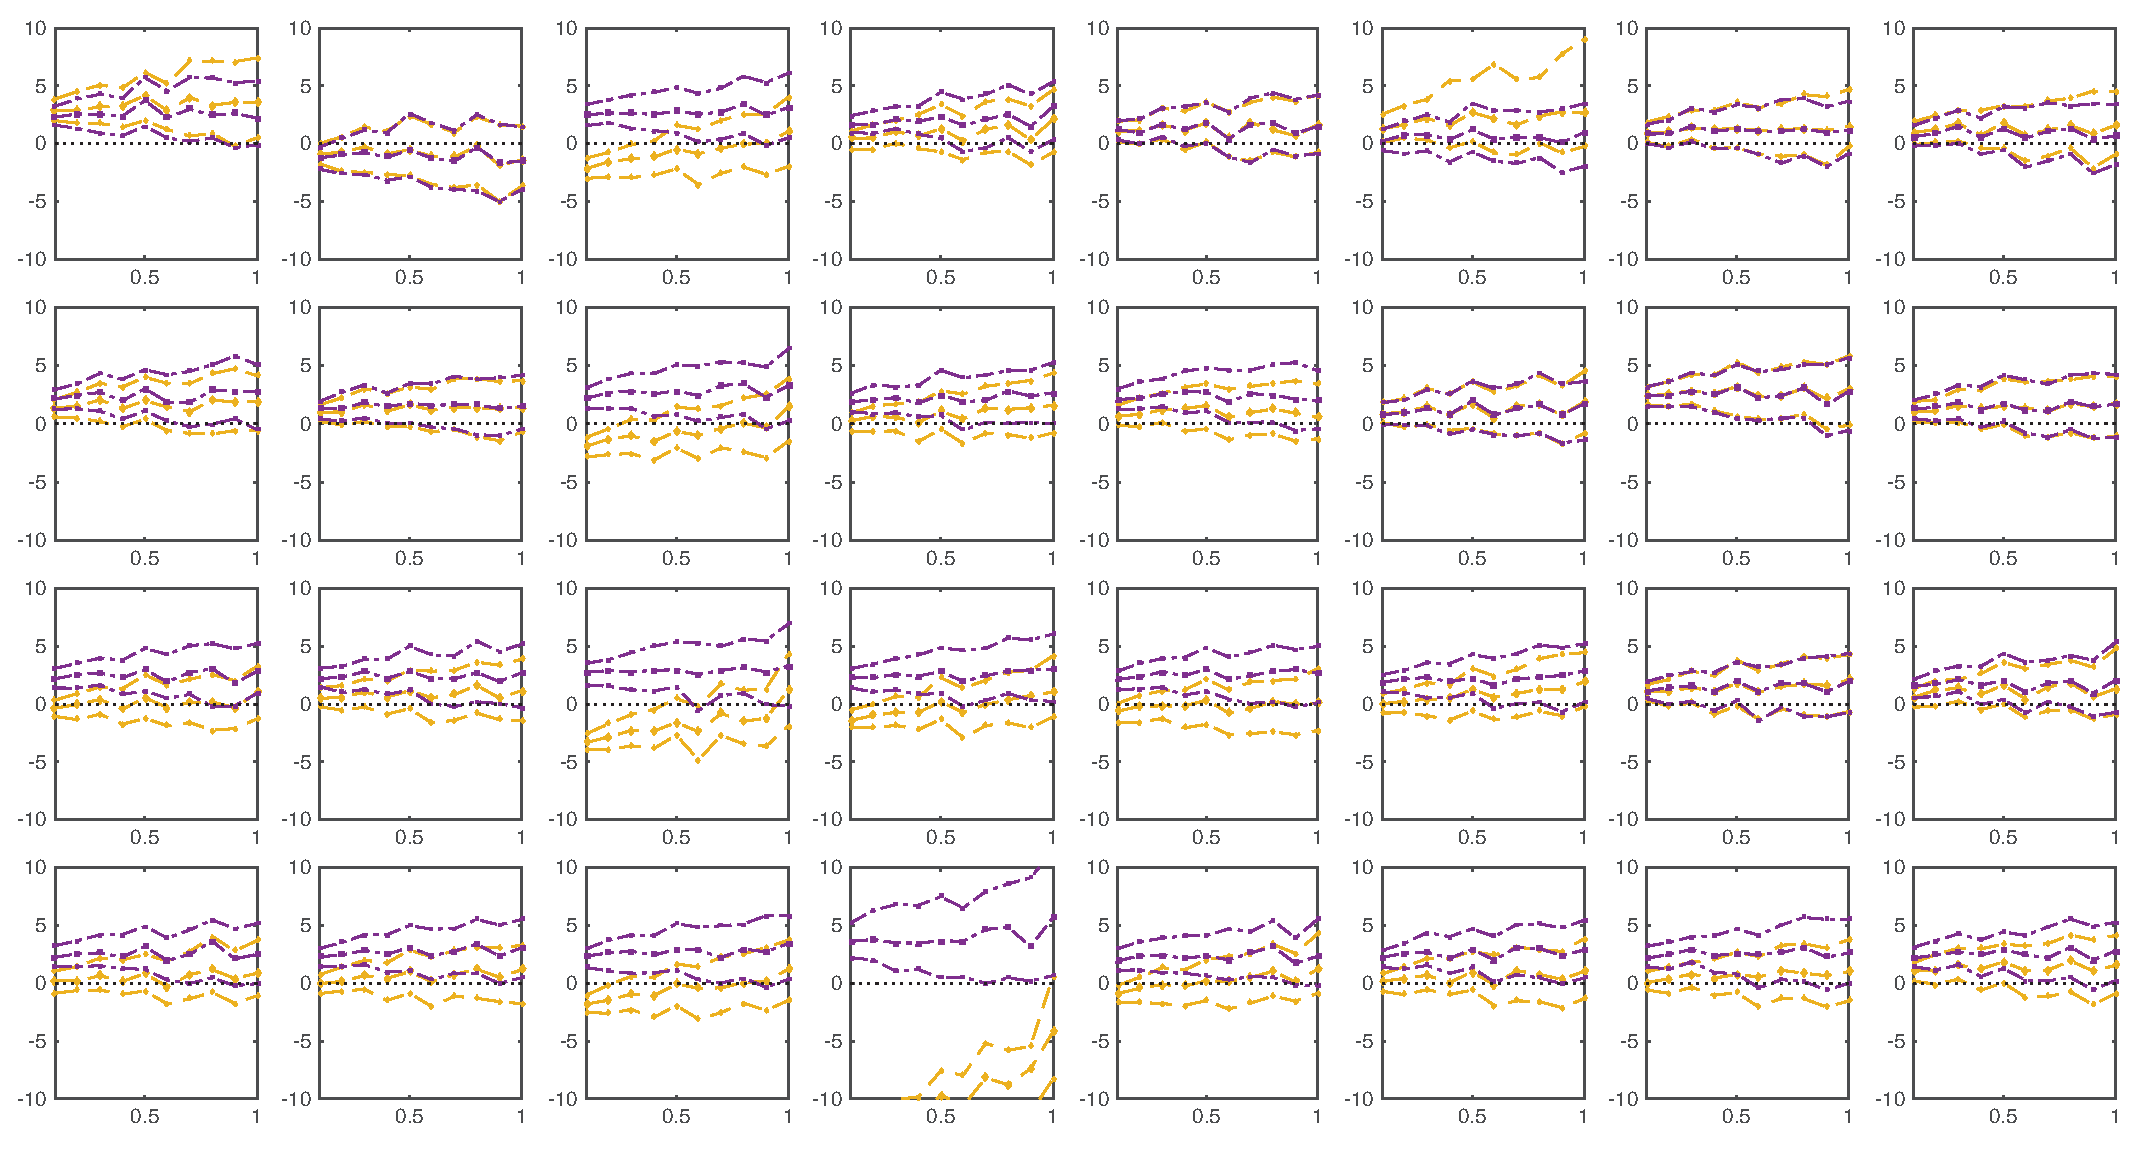
\includegraphics[width=\linewidth]{simSampling_rV.eps}
\caption{Median (large symbols) and first and third quartiles (small symbols) of the relative estimation error for the relative tissue blood volume ($rV$) estimated using the \textbf{rLin} (yellow diamonds) and \textbf{rReg} (purple squares) models, depending on the sampling period used for simulation.}
\label{fig:sampling_rV}
\end{figure}

\begin{figure}
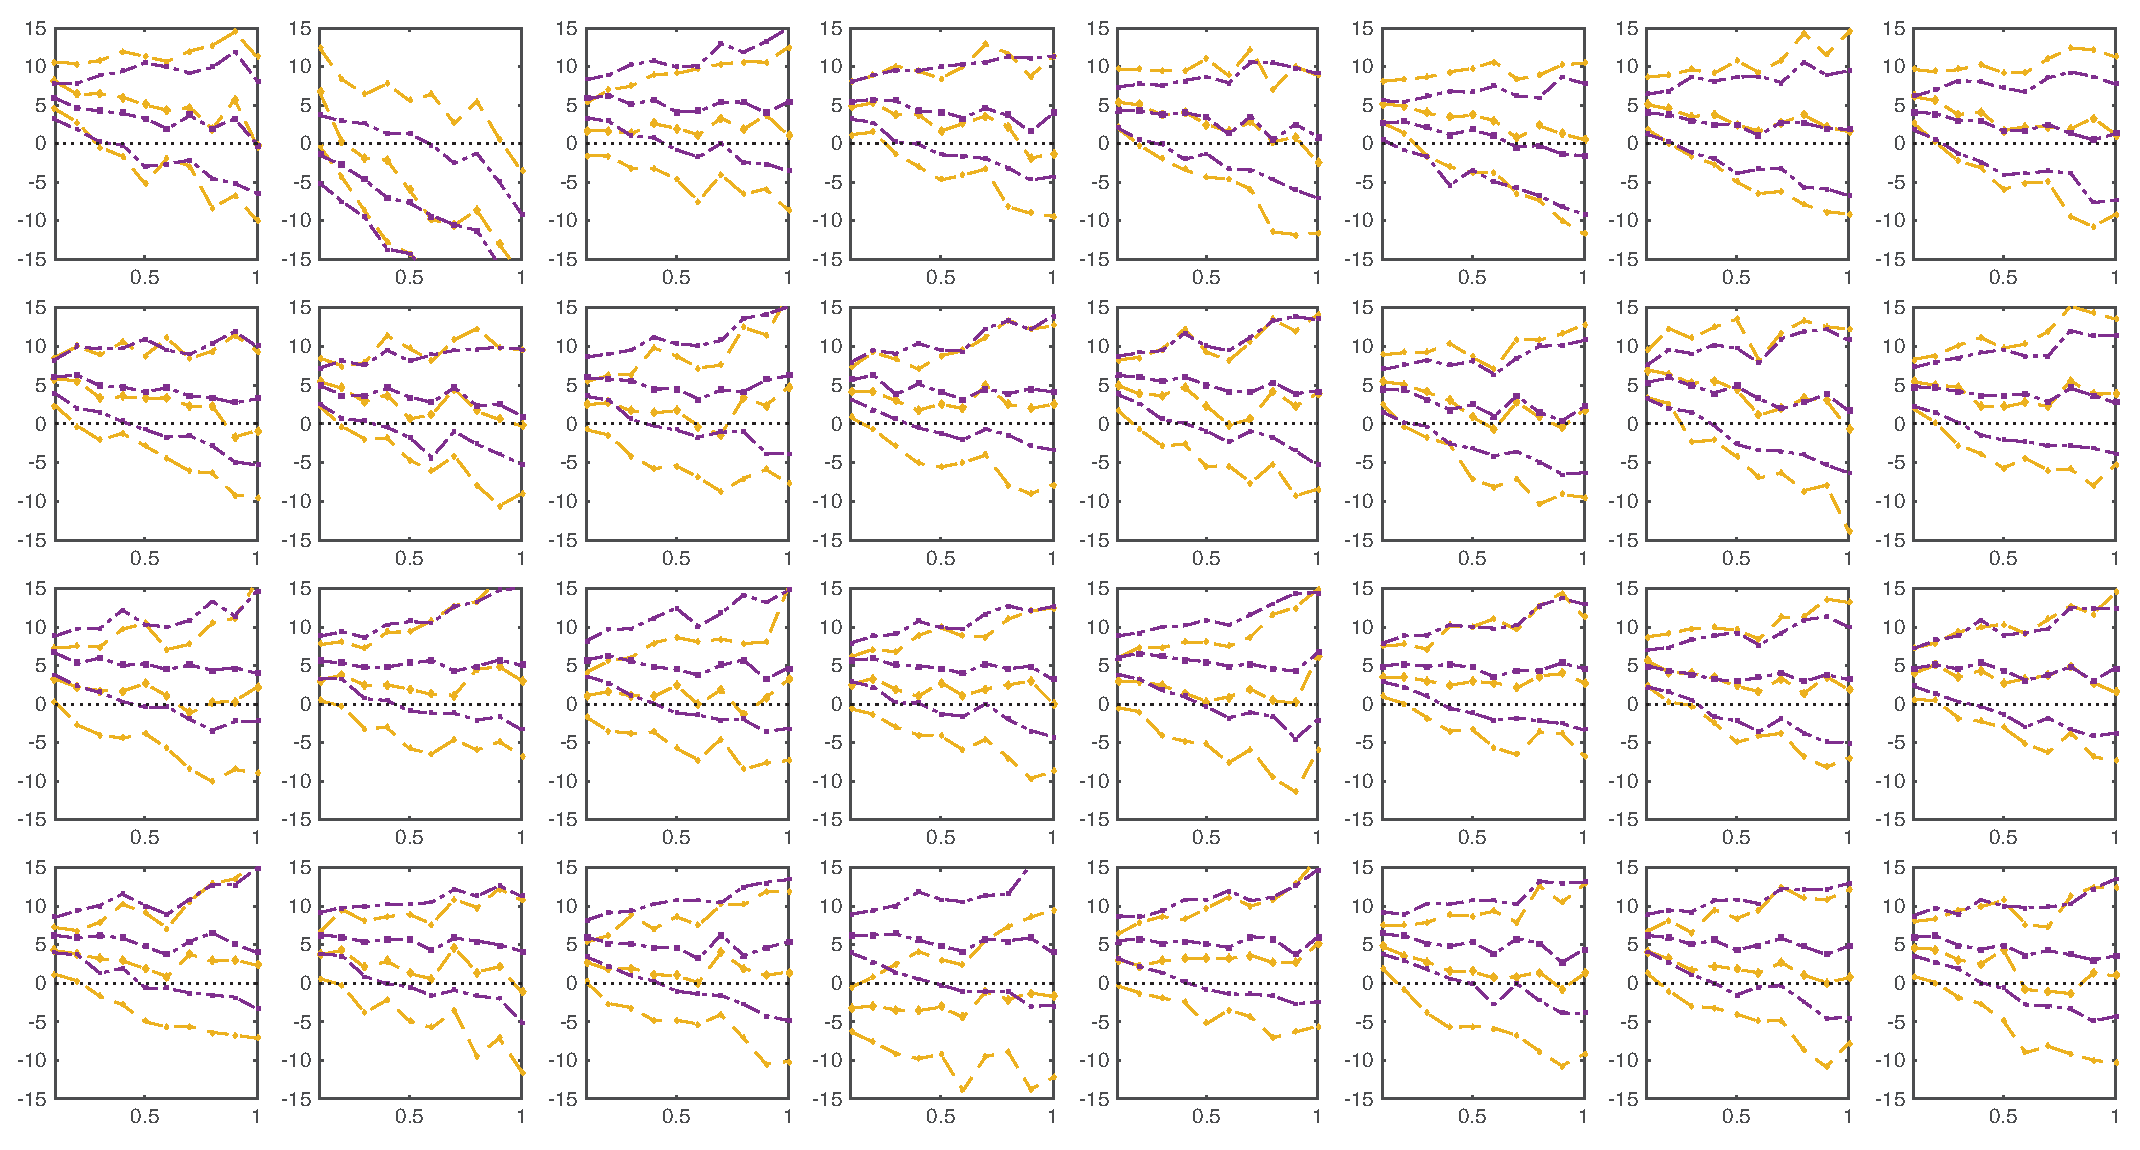
\includegraphics[width=\linewidth]{simSampling_rF.eps}
\caption{Median (large symbols) and first and third quartiles (small symbols) of the relative estimation error for the relative tissue blood flow ($rF$) estimated using the \textbf{rLin} (yellow diamonds) and \textbf{rReg} (purple squares) models, depending on the sampling period used for simulation.}
\label{fig:sampling_rF}
\end{figure}

\begin{figure}
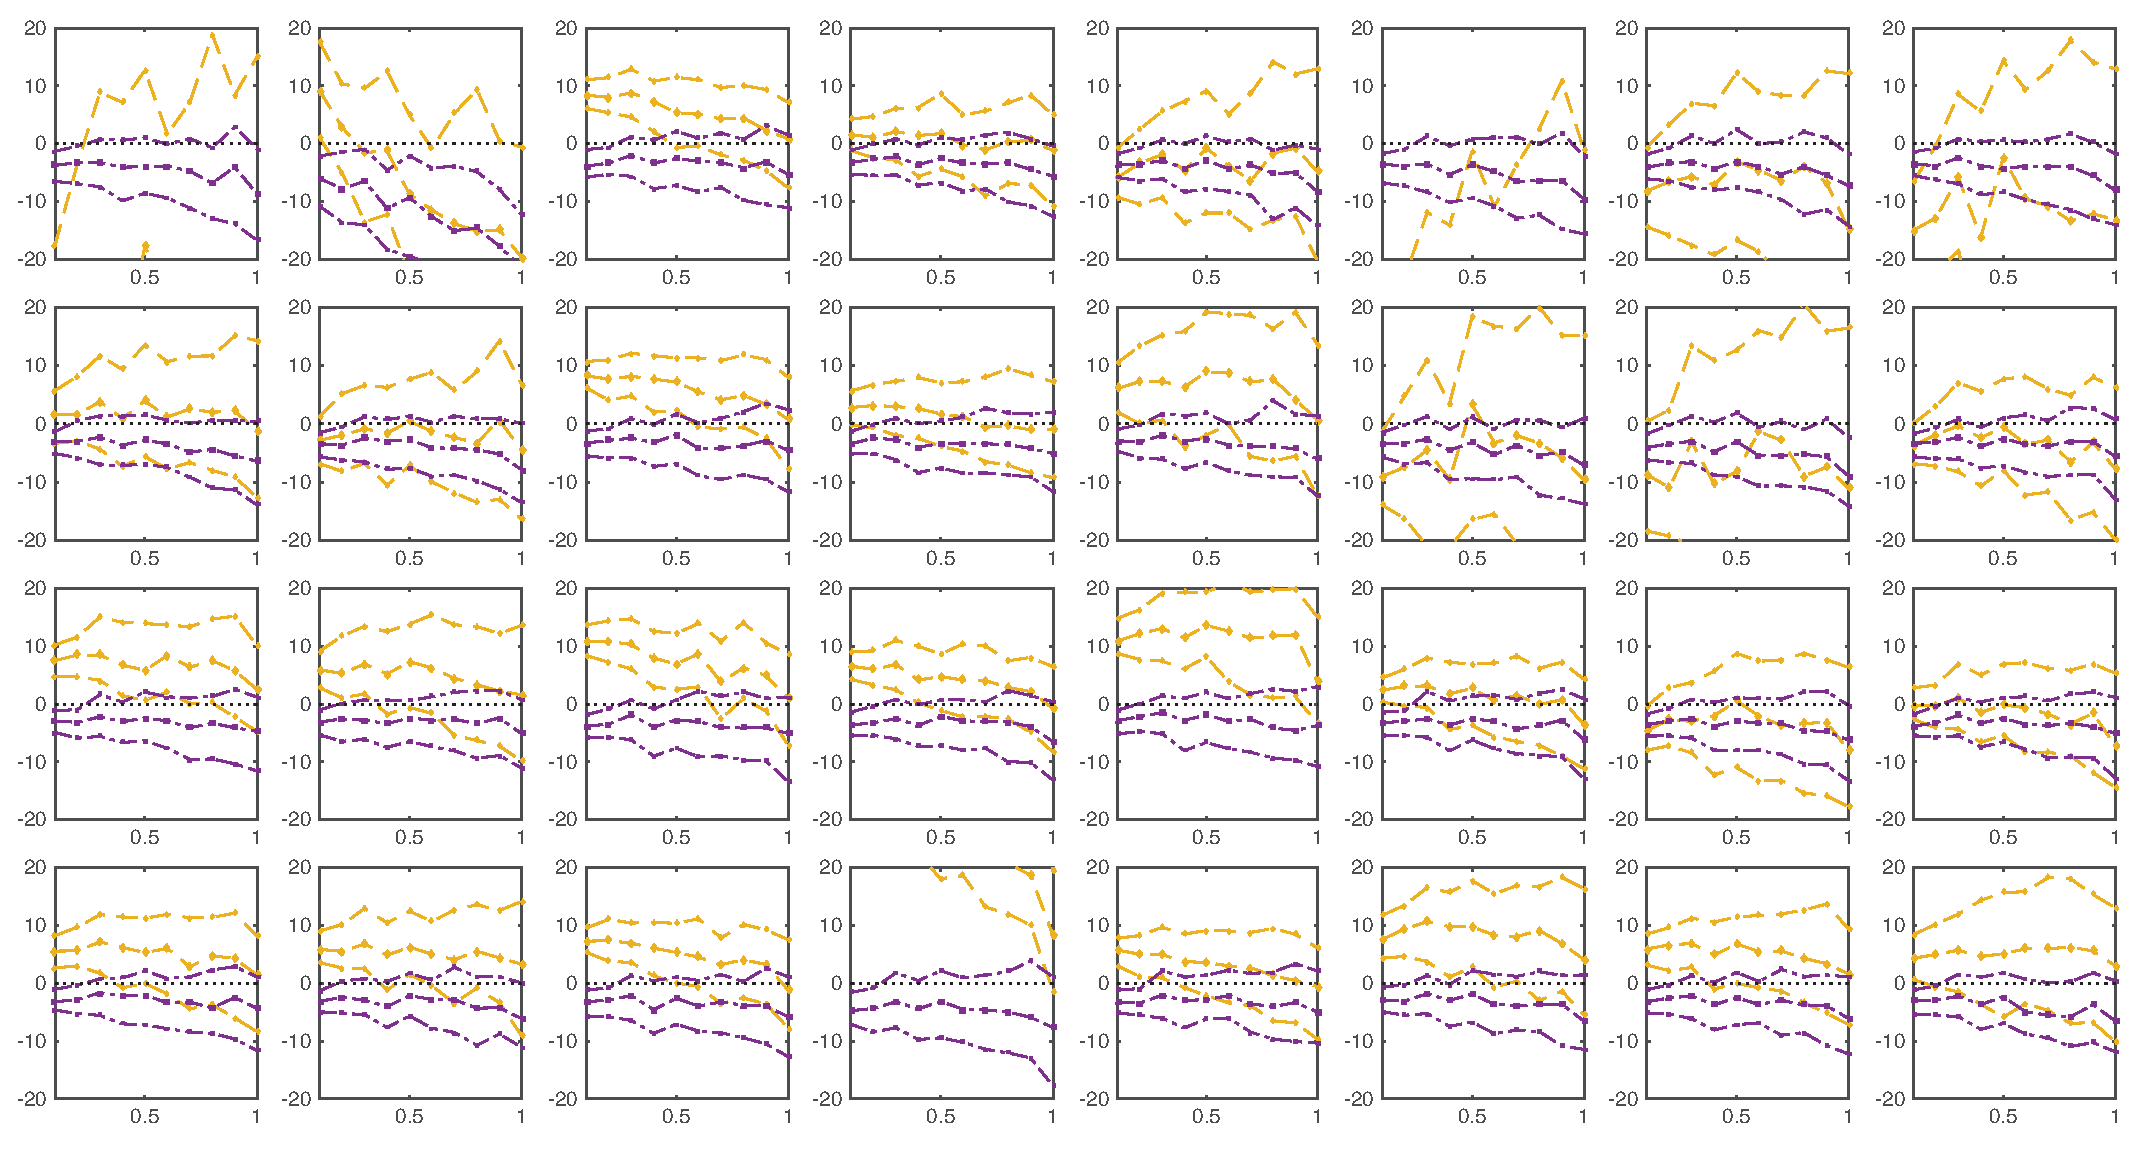
\includegraphics[width=\linewidth]{simSampling_kT.eps}
\caption{Median (large symbols) and first and third quartiles (small symbols) of the relative estimation error for the rate constant in the tumor ($k_T$) estimated using the \textbf{rLin} (yellow diamonds) and \textbf{rReg} (purple squares) models, depending on the sampling period used for simulation.}
\label{fig:sampling_kT}
\end{figure}

\begin{figure}
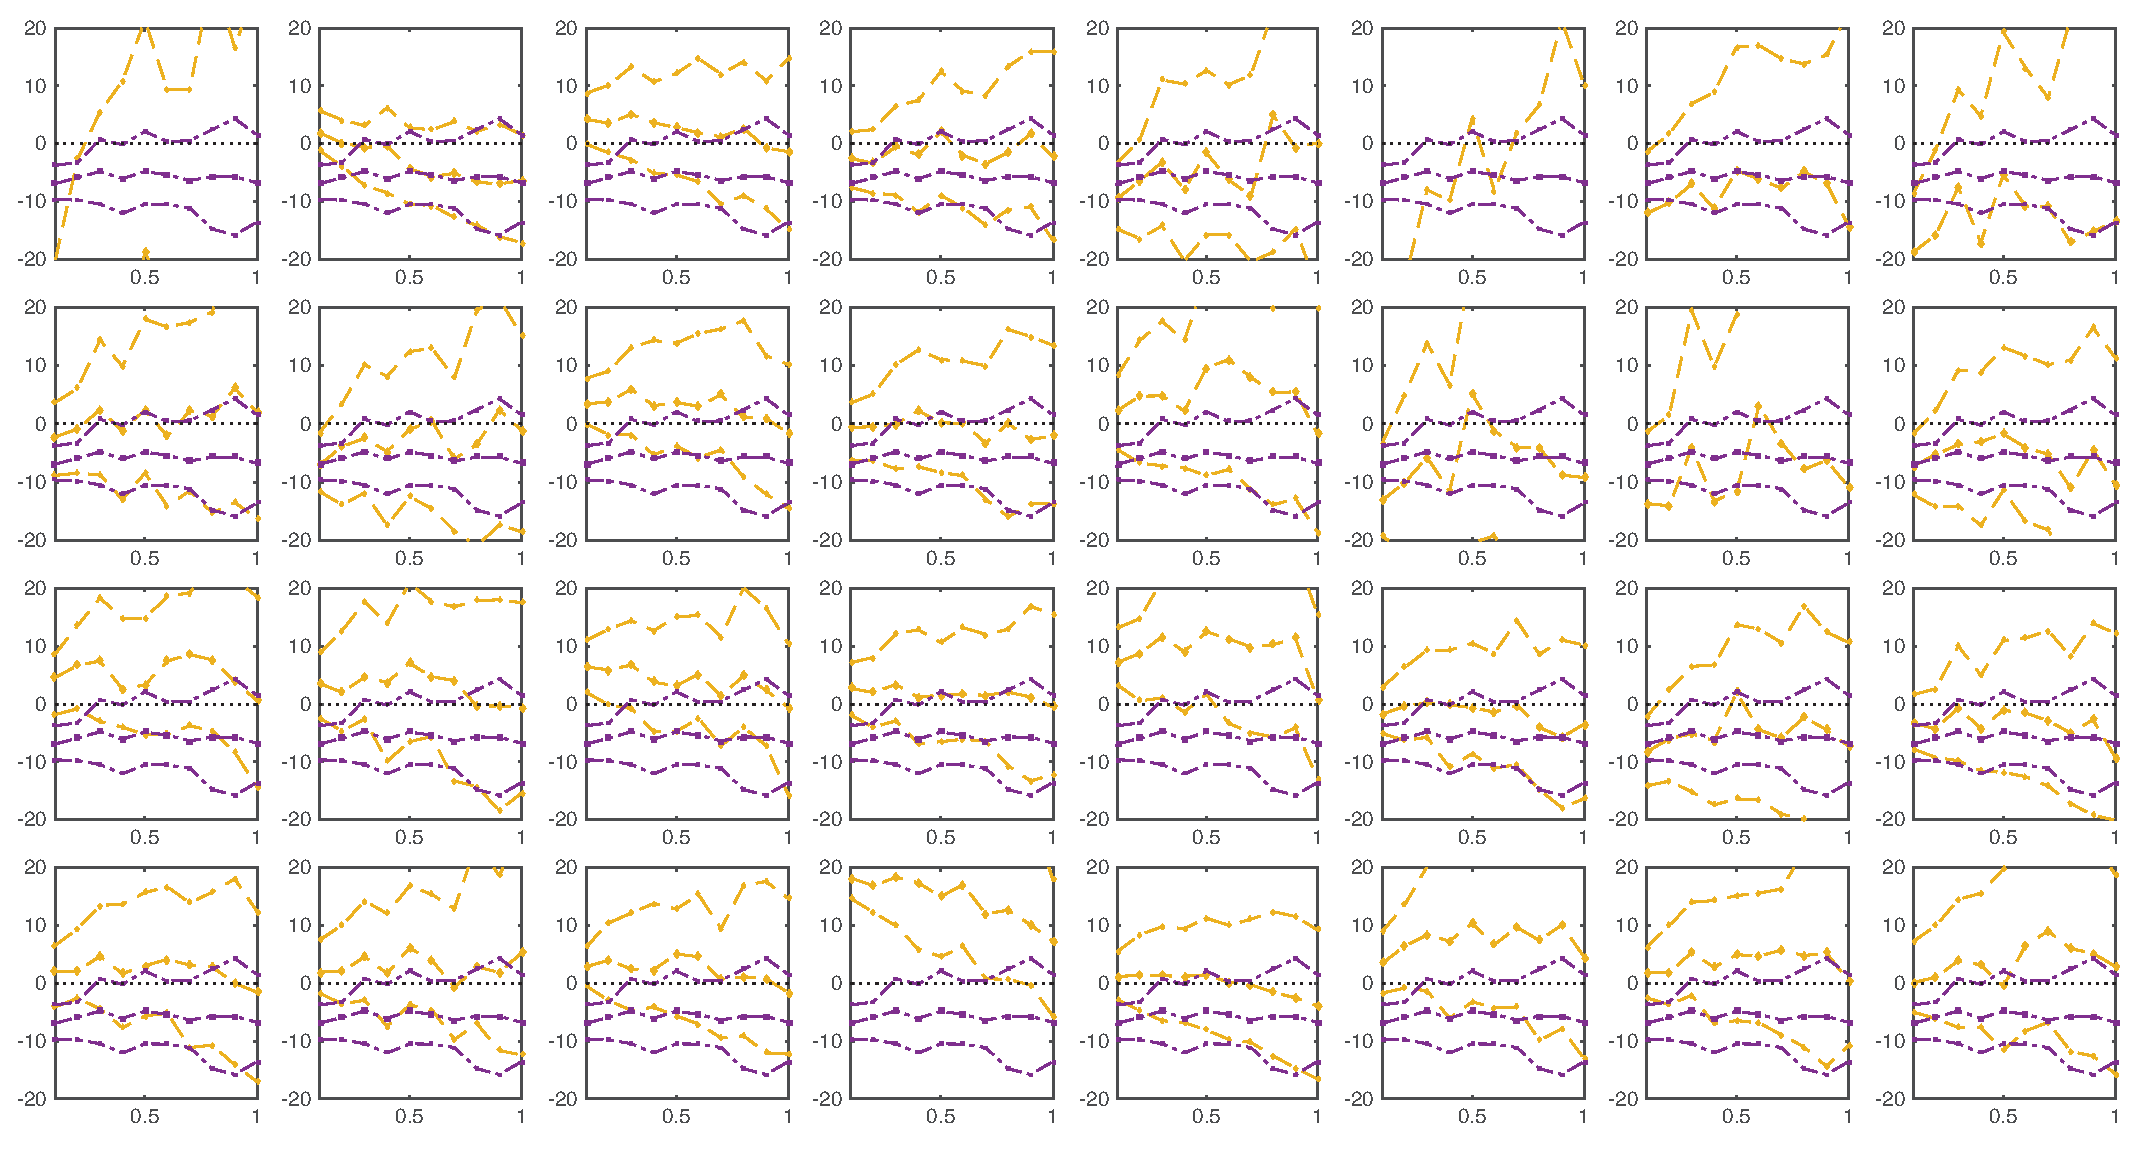
\includegraphics[width=\linewidth]{simSampling_kR.eps}
\caption{Median (large symbols) and first and third quartiles (small symbols) of the relative estimation error for the rate constant in the reference tissue ($k_R$) estimated using the \textbf{rLin} (yellow diamonds) and \textbf{rReg} (purple squares) models, depending on the sampling period used for simulation.}
\label{fig:sampling_kR}
\end{figure}

\paragraph{Reference tissue}
The effect of varying the characteristics of the reference tissue on the accuracy and precision of the estimation process are displayed in Figures~\ref{fig:referenceTissue_rV} to~\ref{fig:referenceTissue_kR}. 
In any of these eight Figures, the first line corresponds to fixed values of the tissue blood volume $V_R$ with varying tissue blood flow $F_R$, the second line corresponds to fixed values of $F_R$ with varying $V_R$, and the third line correspond to fixed values of $k_R$ with varying values of both $V_R$ and $k_R$.
Each bullseye displays the median relative estimation error in each of the 32 tumor regions for the considered parameter.

The relative tissue blood volume (see Figure~\ref{fig:referenceTissue_rV}), $rV$, estimated using the \textbf{rLin} model revealed sensitive to variations of parameter $k_R$.
Indeed, an increase in $k_R$ resulted in increased positive or negative biases, along with increased heterogeneity of the bias across regions.
Using the \textbf{rReg} model reduced the discrepencies across regions compared to the \textbf{rLin} model, but varying $k_R$ one way or the other overestimated the values of $rV$.
Similarly, the relative blood flow (see Figure~\ref{fig:referenceTissue_rF}), $rF$, estimated using either the \textbf{rLin} model or the \textbf{rReg} model were sensitive to variations of $k_R$. 
Larger biases were found using the \textbf{rReg} model, however larger discrepencies across regions were observed in the estimation biases of the \textbf{rLin} model.
For both models, regions with large simulated $k_T$ values were inversely biased, i.e.~$rF$ was underestimated while the other regions were overestimated and oppositely.
The smallest biases in the estimation of $rF$ were found for two thirds of the original $k_R$ value.
In case of fixed $k_R$ values, using lower values of both $F_R$ and $V_R$ yielded overestimated $rV$ and $rF$ values using both models.
Regarding the rate constant in the tumor (see Figure~\ref{fig:referenceTissue_kT}), $k_T$, large discrepencies can be observed using the \textbf{rLin} model, and they tend to increase with decreasing values of $k_R$.
Using the \textbf{rReg} model, the bias in the estimation of $k_T$ increased for lower values of $k_R$.
Additionally, discrepencies across regions are almost inexistant using the \textbf{rReg} model, except in regions with large simulated $k_T$ values, revealing the effect of regularization.
Biases close to zero were found in most regions simulating the reference tissue curve using two thirds of the original $k_R$ value.
The rate constant in the reference tissue (see Figure~\ref{fig:referenceTissue_kR}), $k_R$, exhibited behaviors extremely similar to those of $k_T$, whether estimated using the \textbf{rLin} model or the \textbf{rReg} model.
In case of fixed $k_R$ values, using lower values of both $F_R$ and $V_R$ yielded underestimated $kT$ and $kR$ values using both models.


\begin{figure}
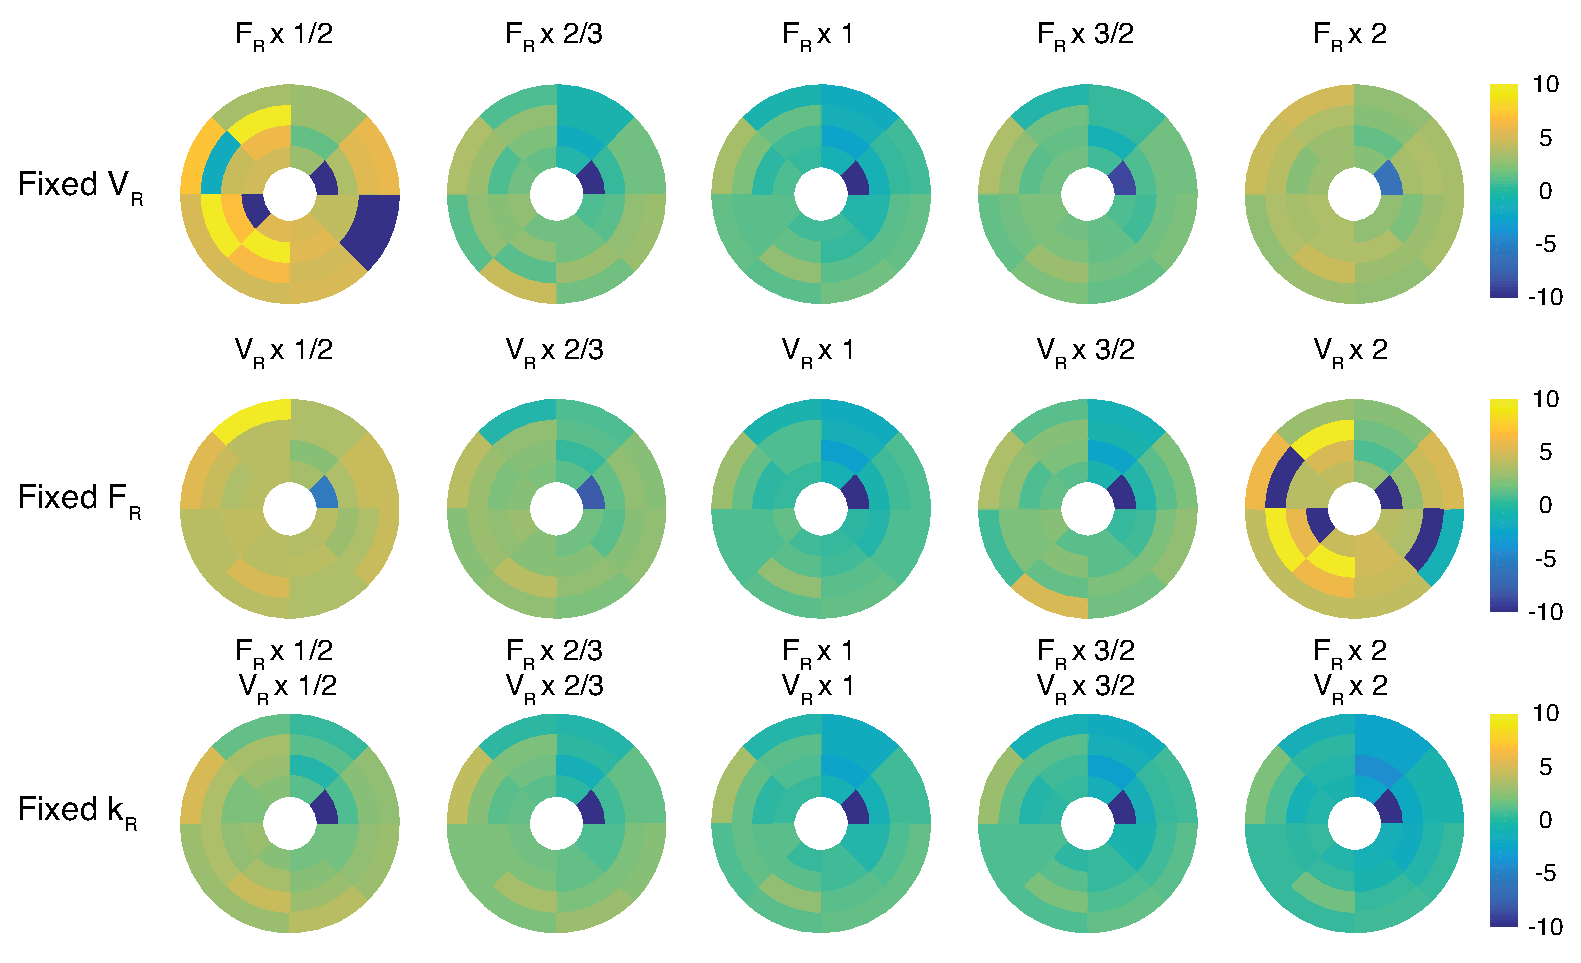
\includegraphics[width=\linewidth]{simRef_rV_rLin.eps}
\par\vspace{1cm}
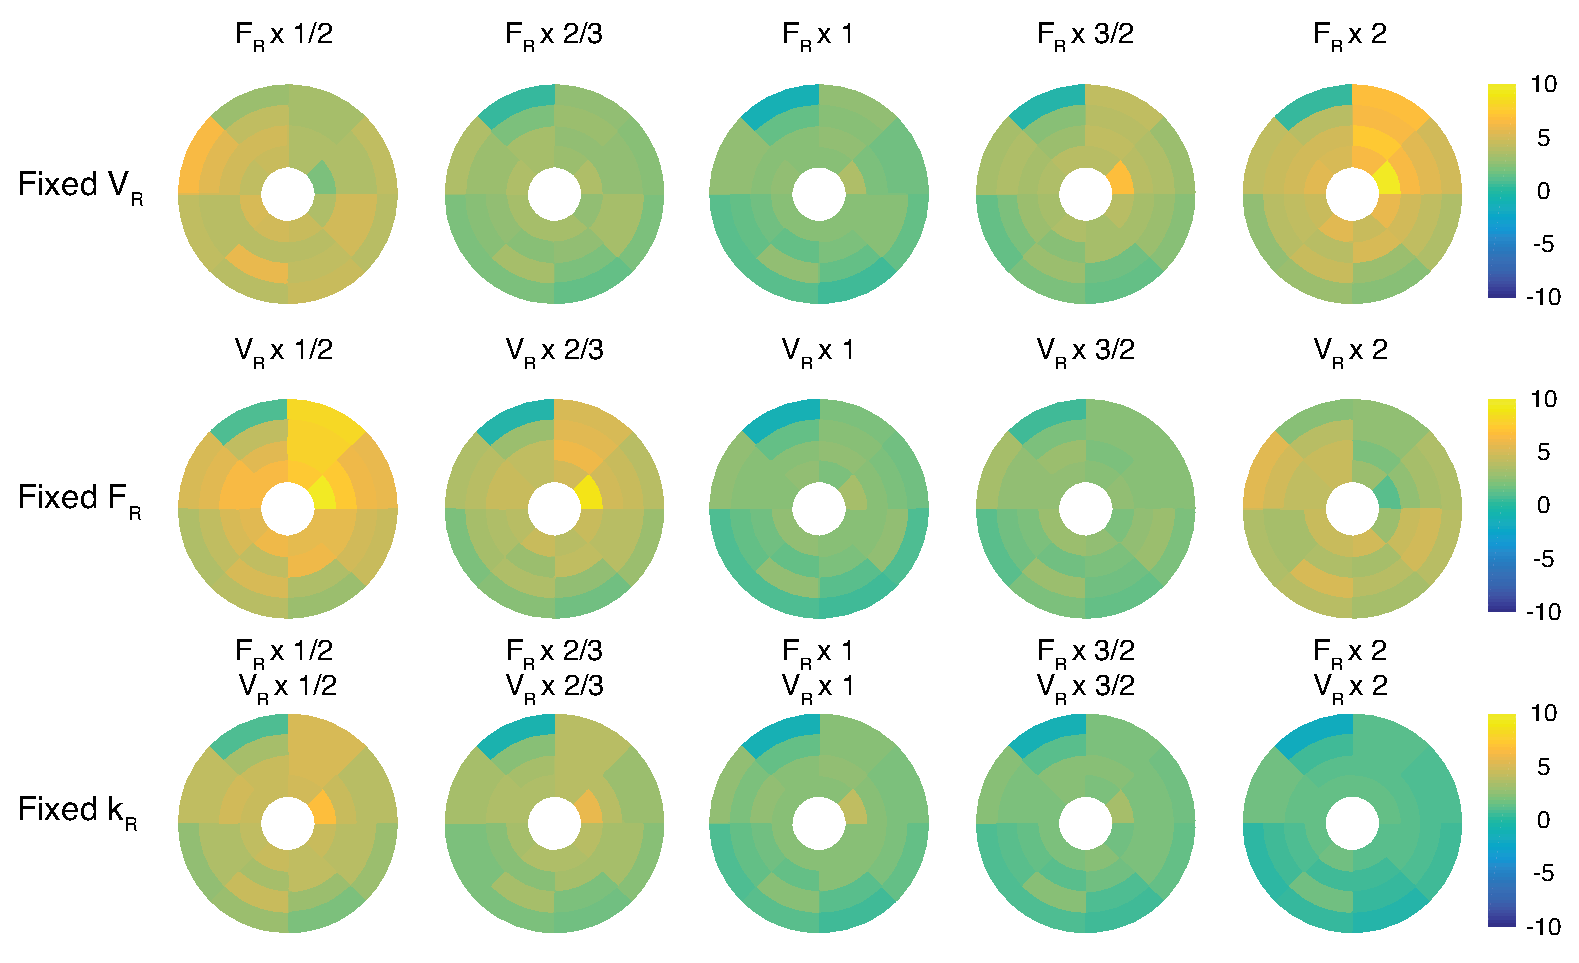
\includegraphics[width=\linewidth]{simRef_rV_rReg.eps}
\caption{Bullseyes of the median relative estimation error for the relative tissue blood volume ($rV$) estimated using the \textbf{rLin} (top) and \textbf{rReg} (bottom) models depending on the characteristics of the reference tissue used for simulation.}
\label{fig:referenceTissue_rV}
\end{figure}

\begin{figure}
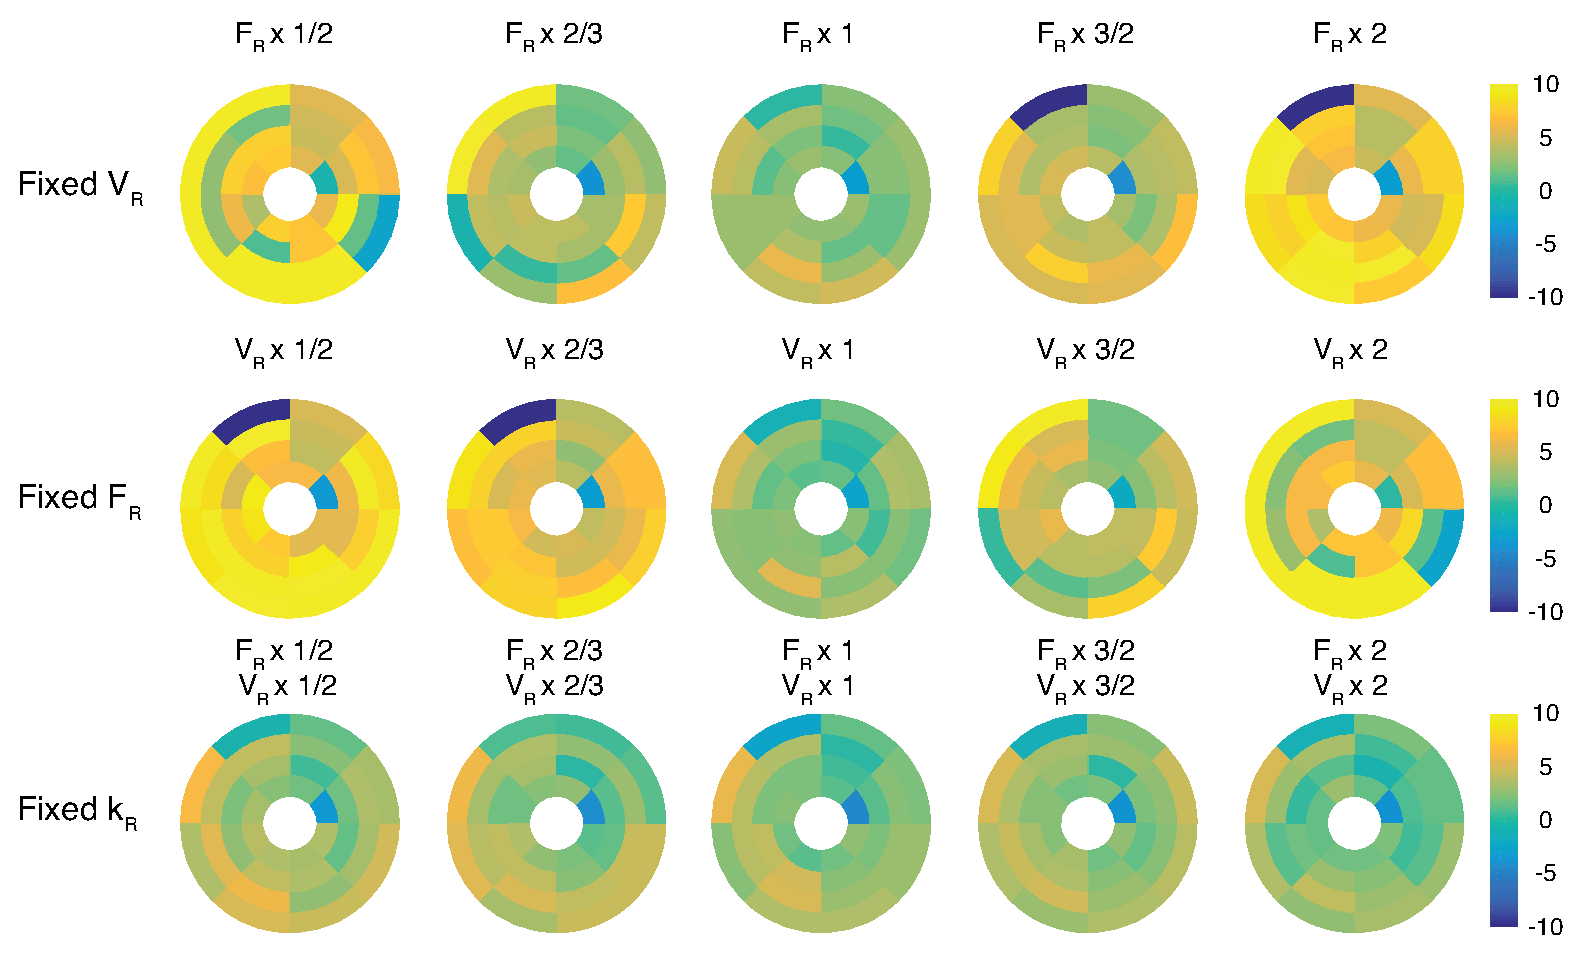
\includegraphics[width=\linewidth]{simRef_rF_rLin.eps}
\par\vspace{1cm}
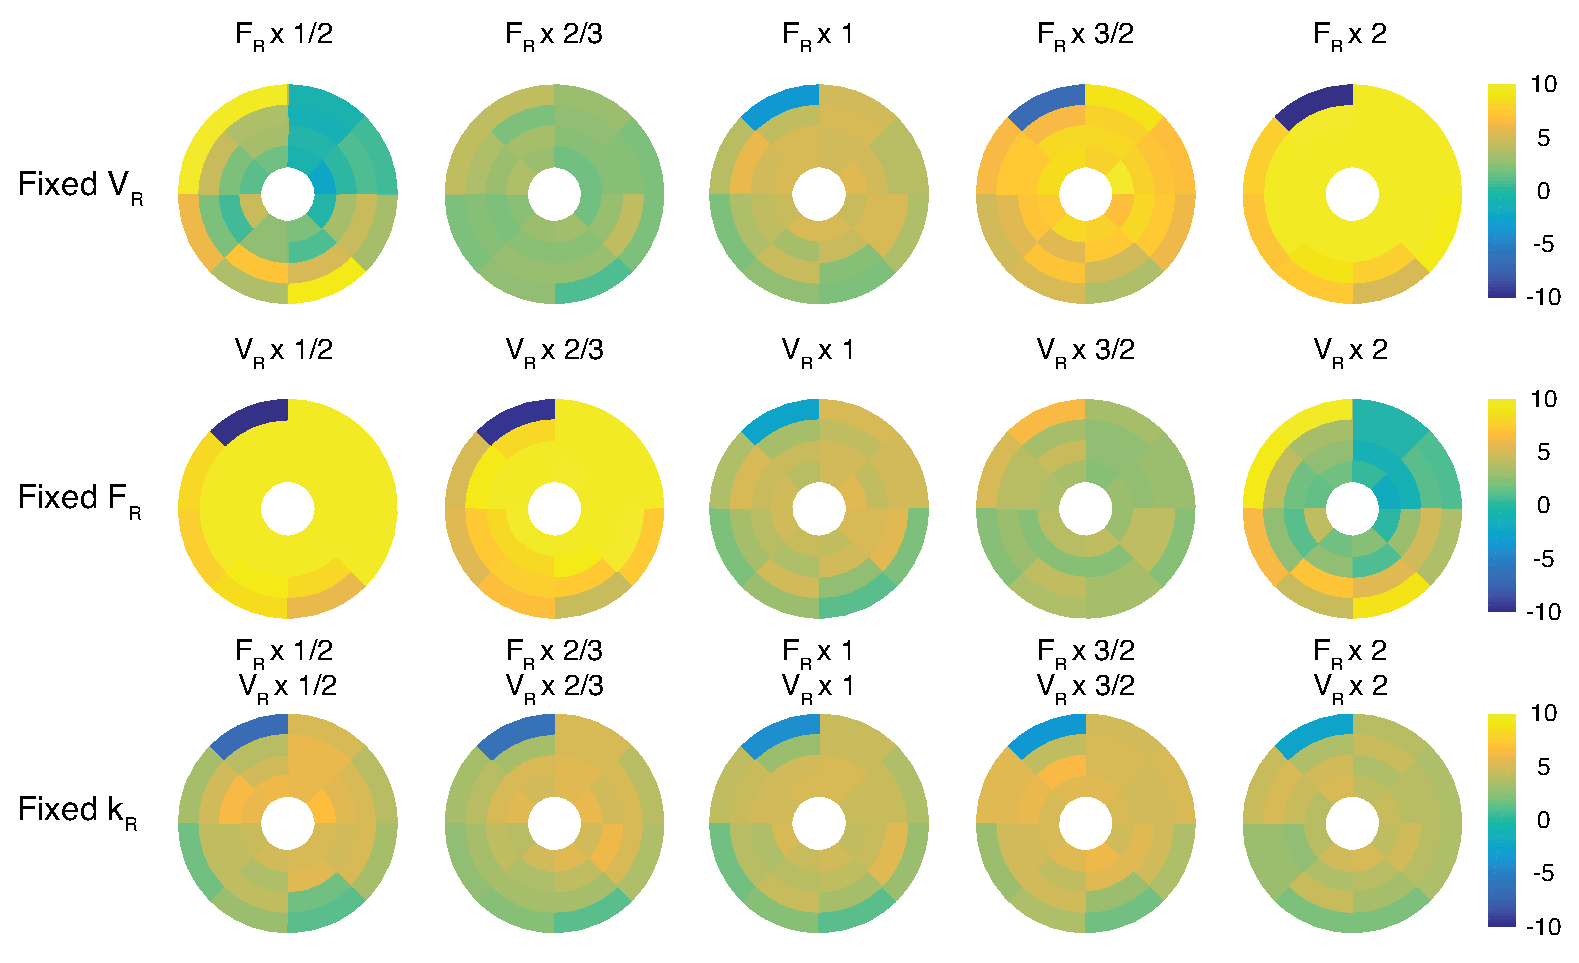
\includegraphics[width=\linewidth]{simRef_rF_rReg.eps}
\caption{Bullseyes of the median relative estimation error for the relative tissue blood flow ($rF$) estimated using the \textbf{rLin} (top) and \textbf{rReg} (bottom) models depending on the characteristics of the reference tissue used for simulation.}
\label{fig:referenceTissue_rF}
\end{figure}

\begin{figure}
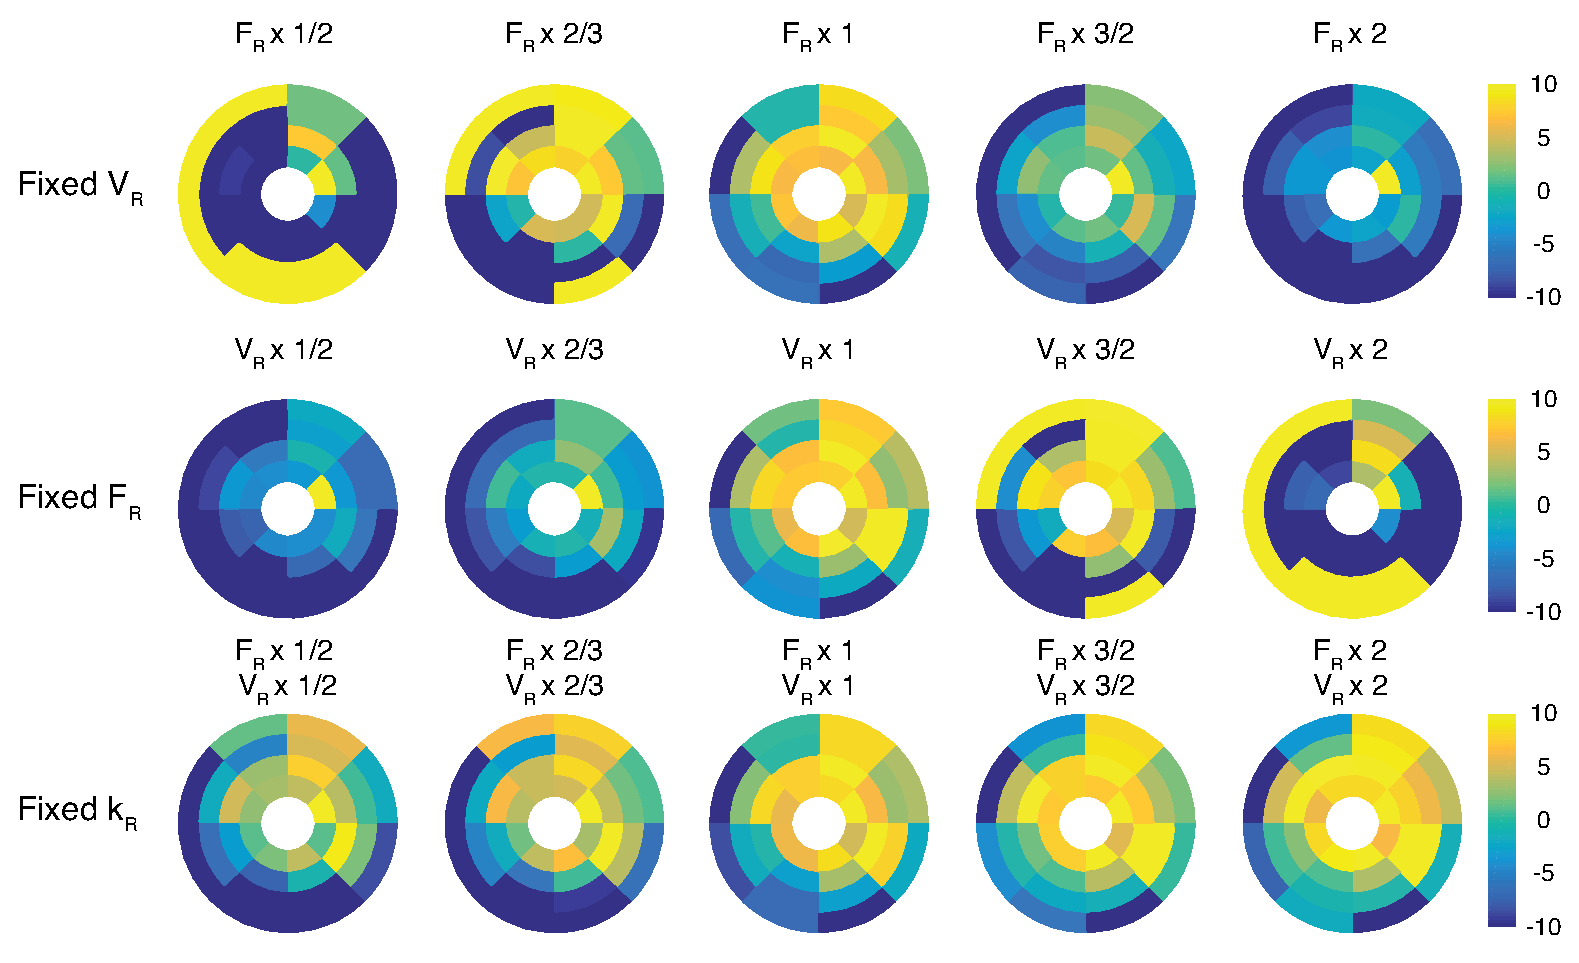
\includegraphics[width=\linewidth]{simRef_kT_rLin.eps}
\par\vspace{1cm}
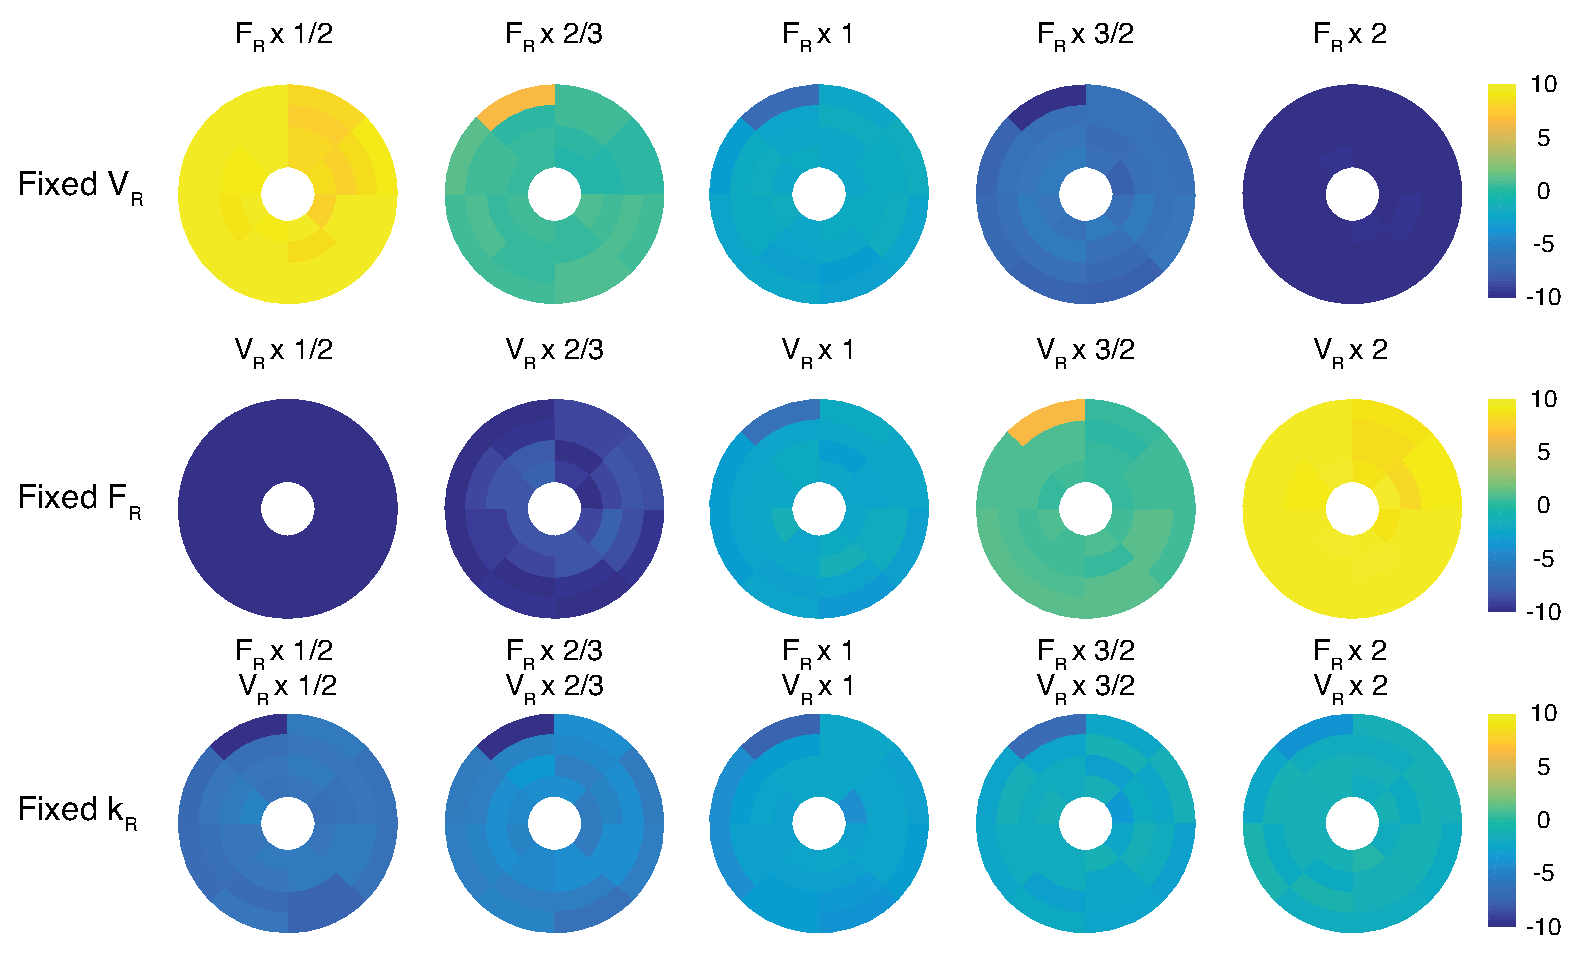
\includegraphics[width=\linewidth]{simRef_kT_rReg.eps}
\caption{Bullseyes of the median relative estimation error for the rate constant in the tumor ($k_T$) estimated using the \textbf{rLin} (top) and \textbf{rReg} (bottom) models depending on the characteristics of the reference tissue used for simulation.}
\label{fig:referenceTissue_kT}
\end{figure}

\begin{figure}
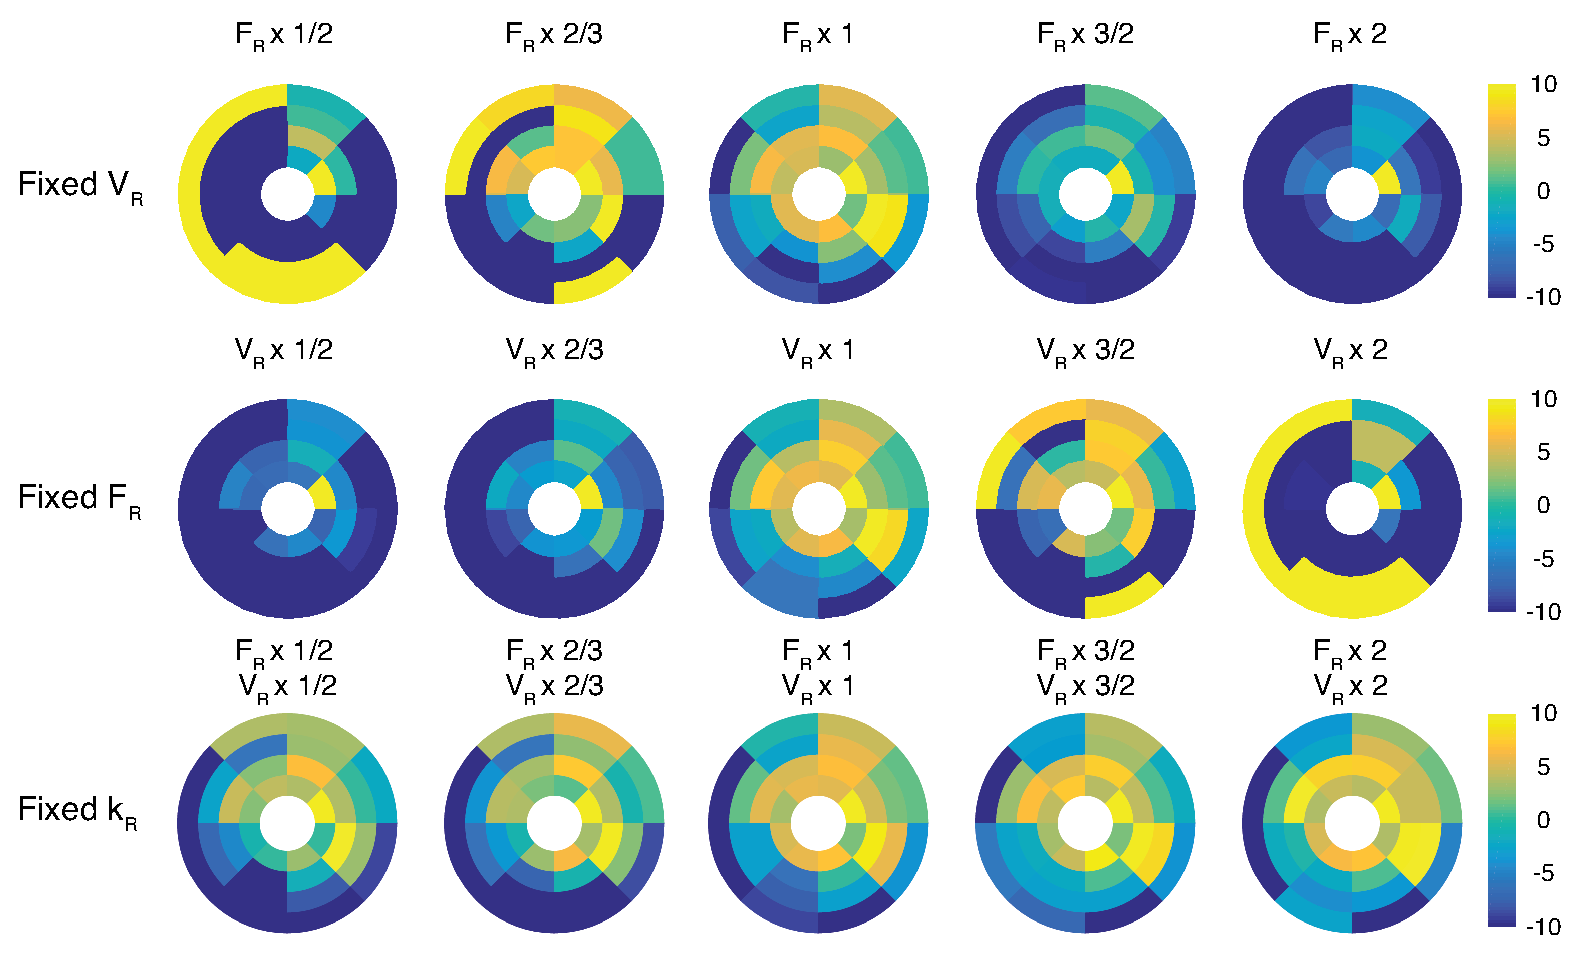
\includegraphics[width=\linewidth]{simRef_kR_rLin.eps}
\par\vspace{1cm}
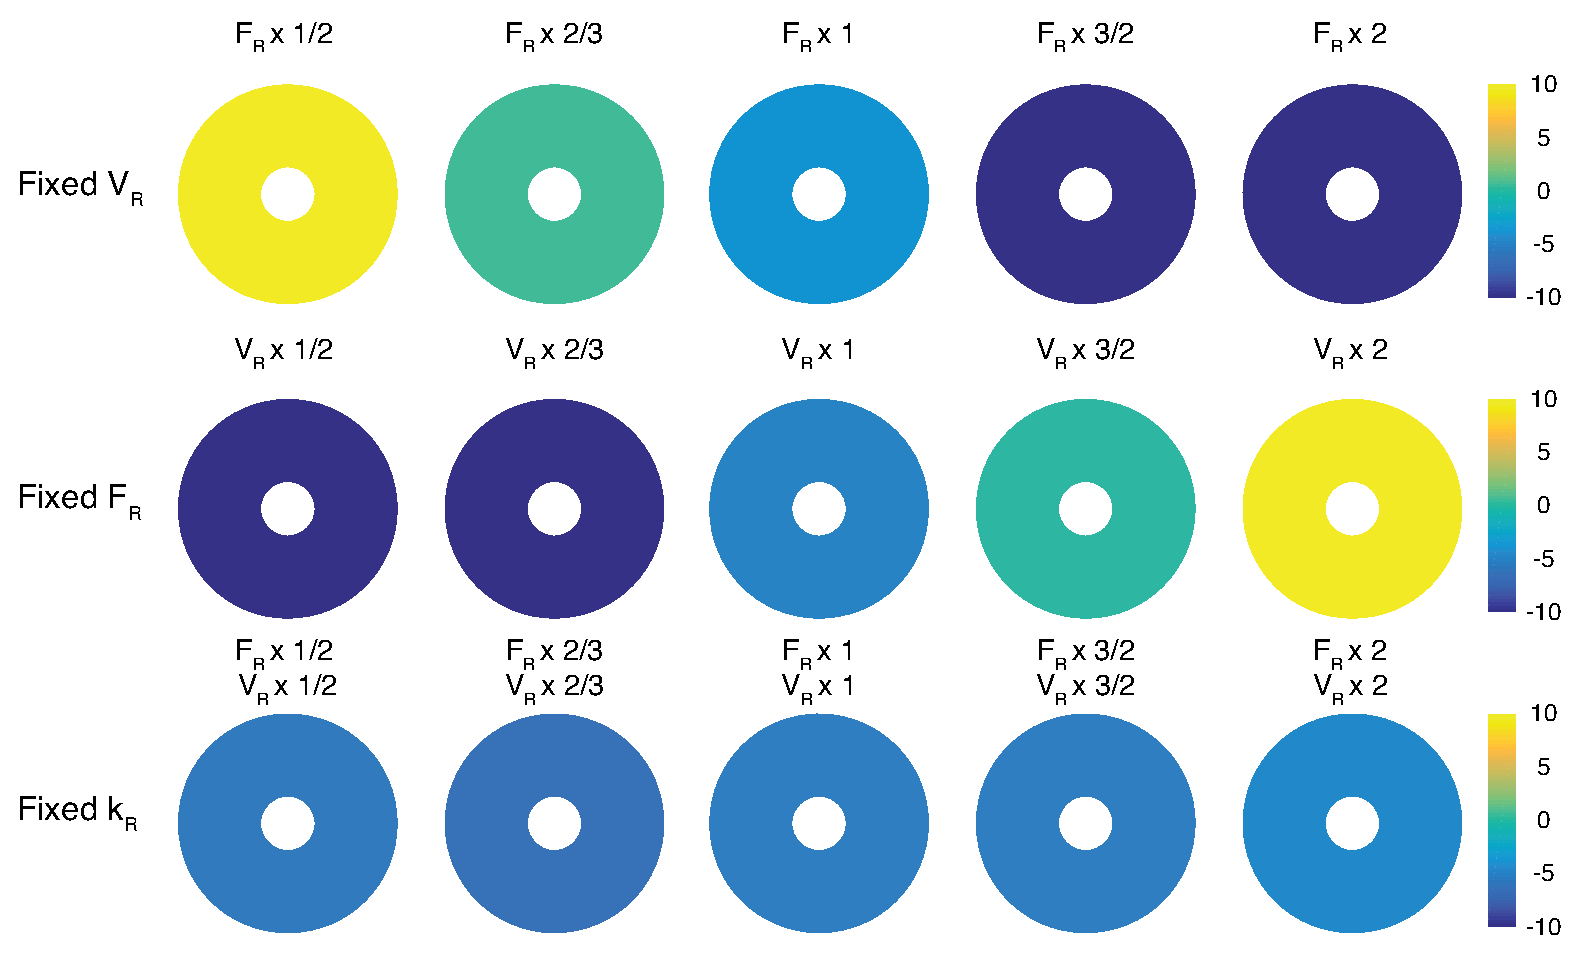
\includegraphics[width=\linewidth]{simRef_kR_rReg.eps}
\caption{Bullseyes of the median relative estimation error for the rate constant in the reference tissue ($k_R$) estimated using the \textbf{rLin} (top) and \textbf{rReg} (bottom) models depending on the characteristics of the reference tissue used for simulation.}
\label{fig:referenceTissue_kR}
\end{figure}


\paragraph{Number of regions}
% Theoretically, the number of regions included in the analysis should not have any impact on the parameter of the \textbf{rLin} model as every kinetic is analyzed individually.
% It should however reveal the importance of regularizing parameter $k_R$ across tumor regions, as introduced by the \textbf{rReg} model, by comparison with the \textbf{rLin} model.
% This study does not account for the variations of the signal to noise ratio depending on the size of the region.
% Instead it investigates solely the impact of the number of regions included in the analysis on the accuracy and precision of the estimates depending on whether the approach is regularized for parameter $k_R$ by keeping the noise level constant regardless of the number of regions.

The impact of varying the number of regions on the accuracy and precision of the estimates of the \textbf{rLin} and \textbf{rReg} models is shown in Figures~\ref{fig:region_rV_rLin} to \ref{fig:region_kR_rReg}.
Indeed, each figure corresponds to a parameter, and the first line represent the accuracy of the estimation through the median relative estimation error, while the second line represent the precision of the estimation through the standard deviation of the relative estimation error.
The relative tissue blood volume $rV$ (see Figure~\ref{fig:region_rV}) from the \textbf{rLin} and \textbf{rReg} models were slightly underestimated using both methods, the latter however yielded more homogeneous median biases across regions.
The \textbf{rLin} model was particularly imprecise in the region exhibiting the larger value of $k_T$.
For both models, no significant effect of the number of region on the accuracy and precision of the estimates of $rV$ was observed in our experiments.
Using the \textbf{rLin} model, increasing the number of region resulted in a lower precision of the regional estimates of $rF$, the relative tissue blood flow (see Figure~\ref{fig:region_rF}).
The \textbf{rReg} model yielded slightly more biased estimates of $rF$, but increasing the number of regions included in the analysis increased the precision of the estimation for studies including two or more regions.
Overall, the biases in the estimates of $rF$ from the \textbf{rReg} model were more consistent across tumor regions.
The rate constant in the tumor $k_T$ (see Figure~\ref{fig:region_kT}) was globally overestimated using the \textbf{rLin} model, except in the region with the largest simulated $k_T$ value where it was underestimated.
The most imprecise estimation of $k_T$ with this model were also found in the four regions exhibiting the largest simulated values of $k_T$.
Using the \textbf{rReg} model considerably reduced the median value of the estimation bias for studies including four or more regions, as well as its standard deviation for studies with eight or more regions.
Additionally, the estimation is more homogeneous acrosse regions in terms of both accuracy and precision.
Regarding $k_R$, the rate constant in the reference tissue (see Figure~\ref{fig:region_kR}), the precision and the homogeneity of the estimates from the \textbf{rLin} model clearly decreases with the number of regions, while the precision actually increases using the \textbf{rReg} model. 
Increasing the number of regions increased the heterogeneity of the biases in the $k_R$ estimates of the \textbf{rLin} model.
The $k_R$ estimates of the \textbf{rReg} model exhibit a slight negative bias, which does not change much when changing the number of regions

\begin{figure}
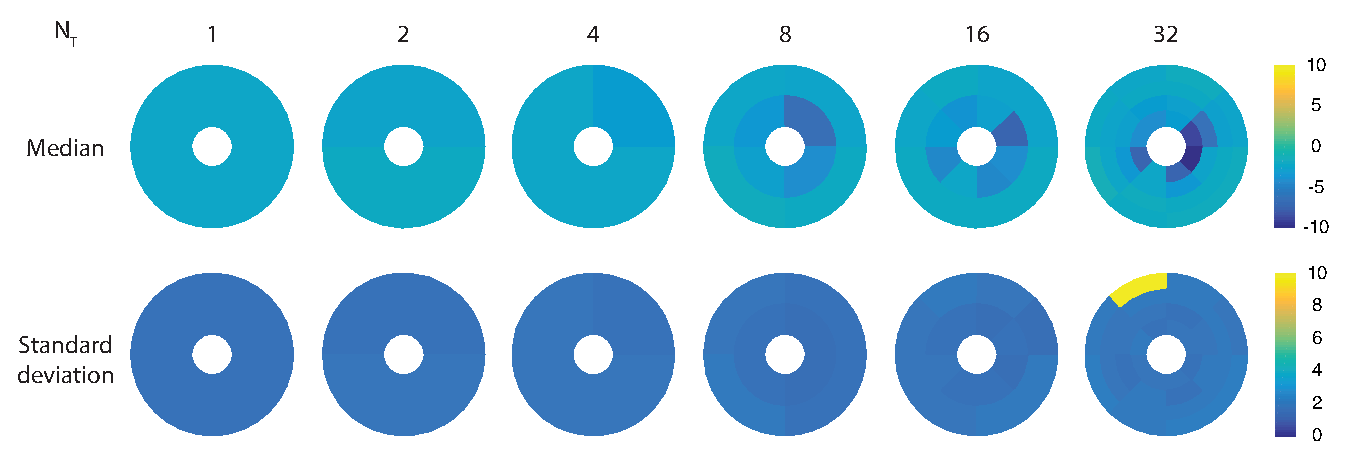
\includegraphics[width=\linewidth]{simReg_rV_rLin.eps}
\par\vspace{1cm}
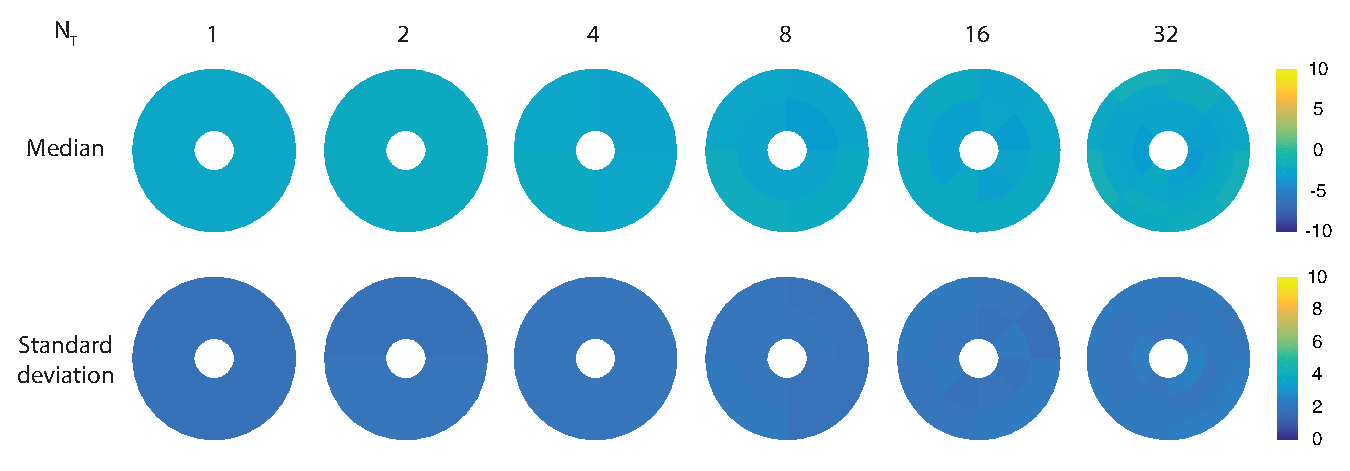
\includegraphics[width=\linewidth]{simReg_rV_rReg.eps}
\caption{Bullseyes of the median value and the standard deviation of the relative estimation error for the relative tissue blood volume ($rV$) estimated using the \textbf{rLin} (top) and \textbf{rReg} (bottom) models depending on the number of regions $N_T$.}
\label{fig:region_rV}
\end{figure}

\begin{figure}
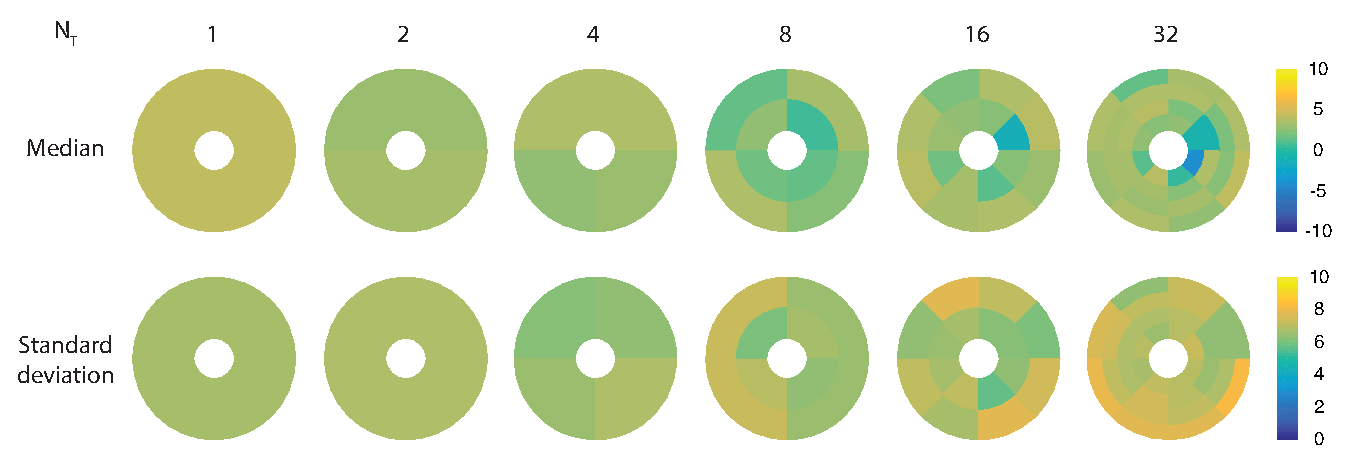
\includegraphics[width=\linewidth]{simReg_rF_rLin.eps}
\par\vspace{1cm}
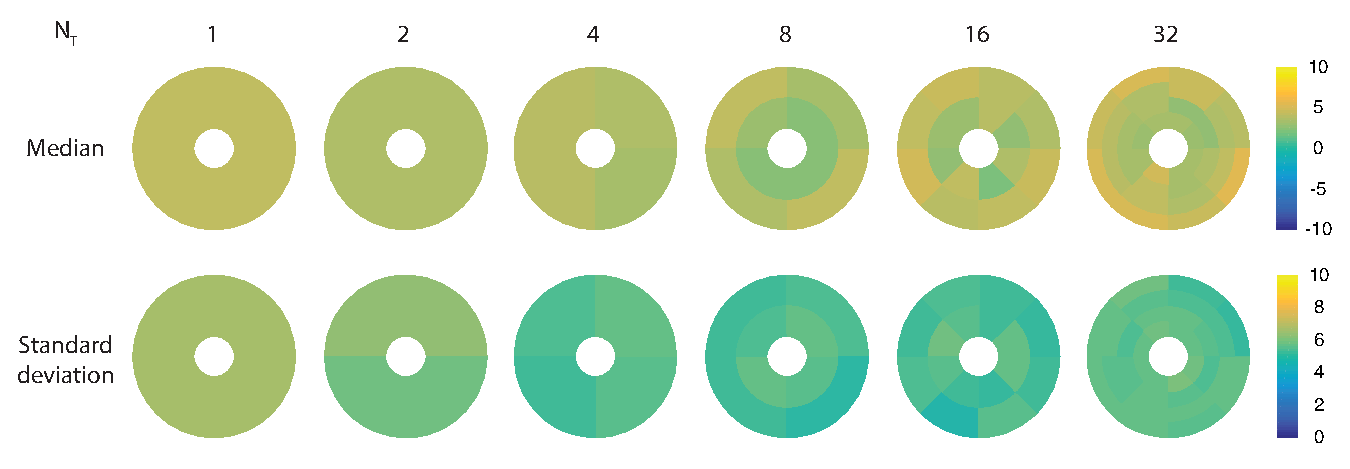
\includegraphics[width=\linewidth]{simReg_rF_rReg.eps}
\caption{Bullseyes of the median value and the standard deviation of the relative estimation error for the relative tissue blood flow ($rF$) estimated using the \textbf{rLin} (top) and \textbf{rReg} (bottom) models depending on the number of regions $N_T$.}
\label{fig:region_rF}
\end{figure}

\begin{figure}
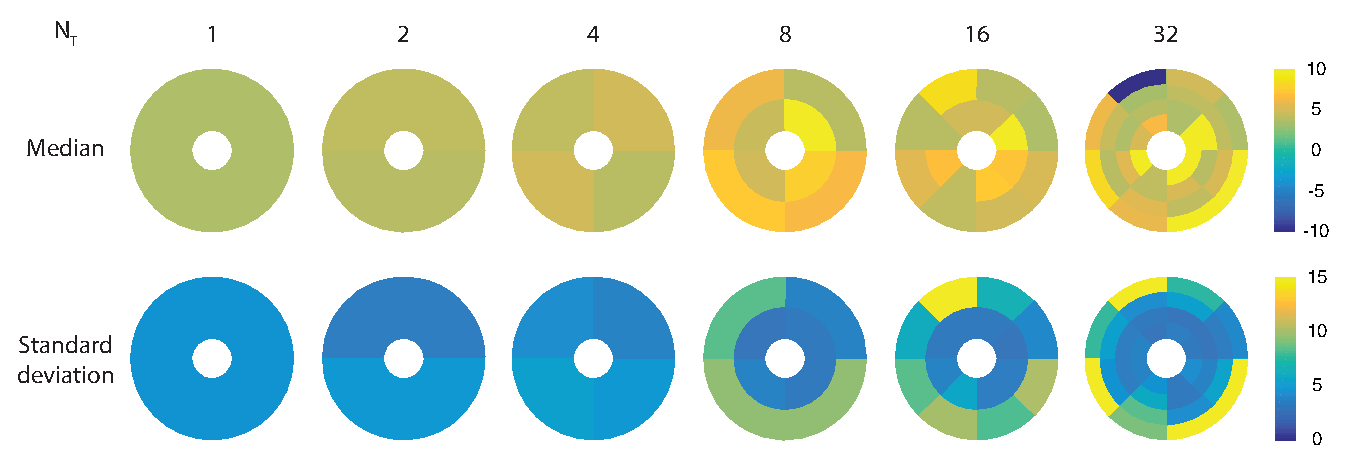
\includegraphics[width=\linewidth]{simReg_kT_rLin.eps}
\par\vspace{1cm}
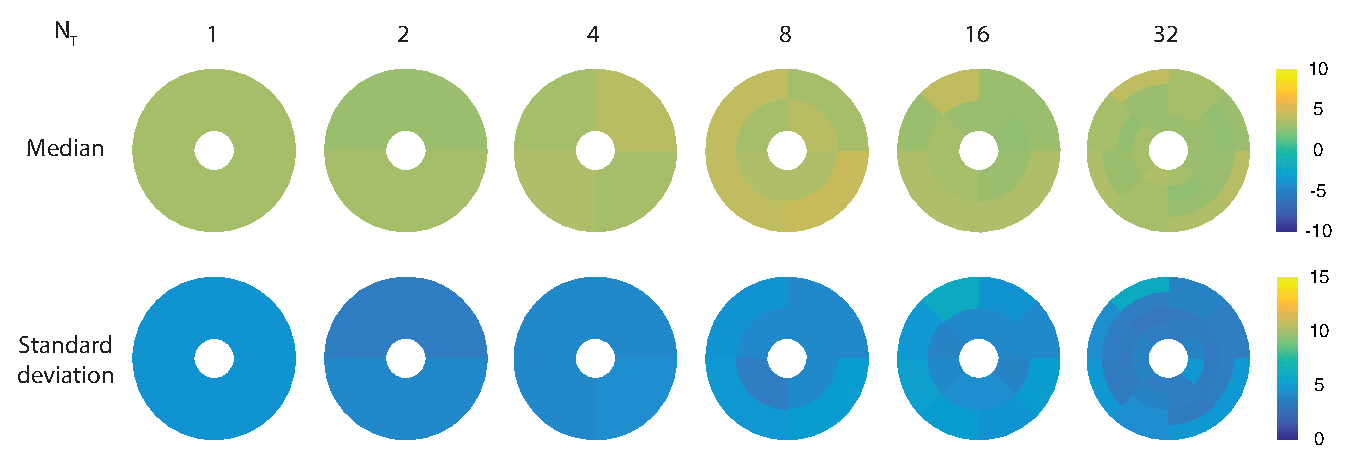
\includegraphics[width=\linewidth]{simReg_kT_rReg.eps}
\caption{Bullseyes of the median value and the standard deviation of the relative estimation error for the rate constant in the tumor ($k_T$) estimated using the \textbf{rLin} (top) and \textbf{rReg} (bottom) models depending on the number of regions $N_T$.}
\label{fig:region_kT}
\end{figure}

\begin{figure}
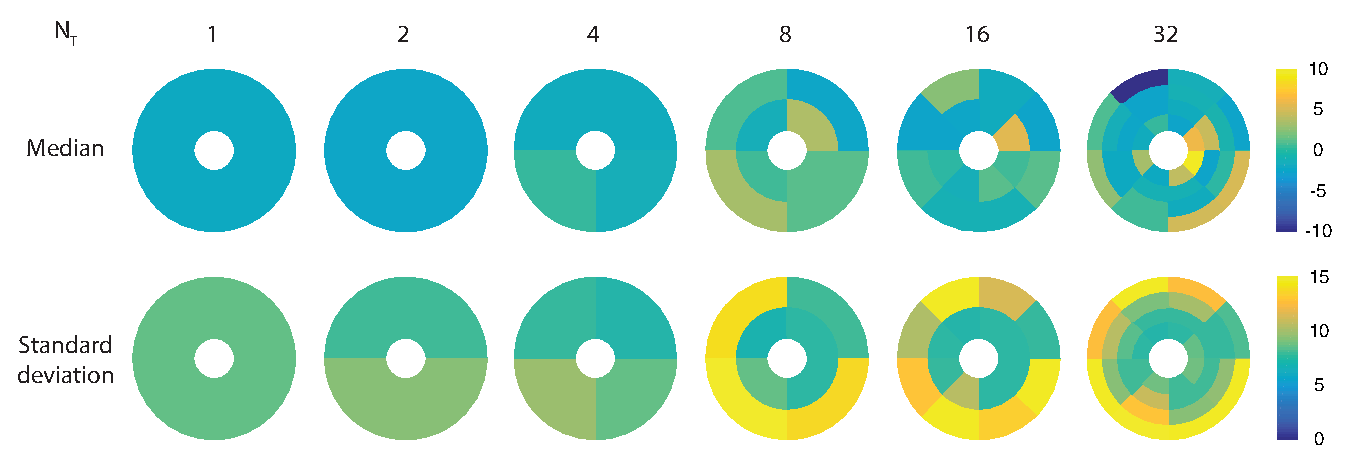
\includegraphics[width=\linewidth]{simReg_kR_rLin.eps}
\par\vspace{1cm}
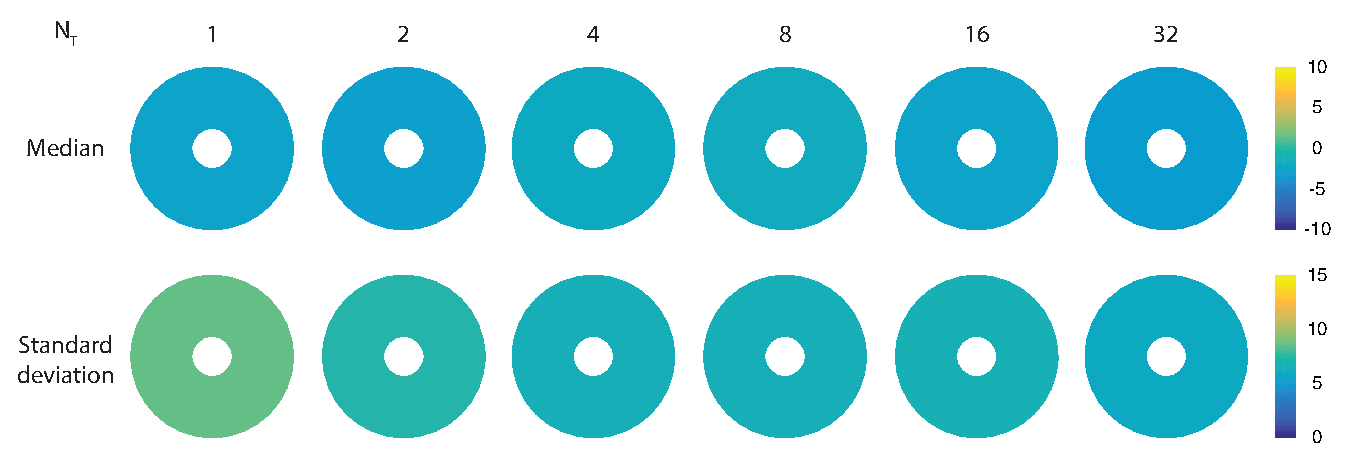
\includegraphics[width=\linewidth]{simReg_kR_rReg.eps}
\caption{Bullseyes of the median value and the standard deviation of the relative estimation error for the rate constant in the reference tissue ($k_R$) estimated using the \textbf{rLin} (top) and \textbf{rReg} (bottom) models depending on the number of regions $N_T$.}
\label{fig:region_kR}
\end{figure}


\section{Discussion}
Nulla mi mi, venenatis sed ipsum varius, volutpat euismod diam. Proin rutrum vel massa non gravida. Quisque tempor sem et dignissim rutrum. Lorem ipsum dolor sit amet, consectetur adipiscing elit. Morbi at justo vitae nulla elementum commodo eu id massa. In vitae diam ac augue semper tincidunt eu ut eros. Fusce fringilla erat porttitor lectus cursus, vel sagittis arcu lobortis. Aliquam in enim semper, aliquam massa id, cursus neque. Praesent faucibus semper libero.

\section{Conclusion}
Sed non aliquet felis. Lorem ipsum dolor sit amet, consectetur adipiscing elit. Mauris commodo justo ac dui pretium imperdiet. Sed suscipit iaculis mi at feugiat. Ut neque ipsum, luctus id lacus ut, laoreet scelerisque urna. Phasellus venenatis, tortor nec vestibulum mattis, massa tortor interdum felis, nec pellentesque metus tortor nec nisl. Ut ornare mauris tellus, vel dapibus arcu suscipit sed. Nam condimentum sem eget mollis euismod. Nullam dui urna, gravida venenatis dui et, tincidunt sodales ex. Nunc est dui, sodales sed mauris nec, auctor sagittis leo. Aliquam tincidunt, ex in facilisis elementum, libero lectus luctus est, non vulputate nisl augue at dolor.